% main.tex -- manuscript source.
%
% Scope: results frozen at Gate G2 (tag results-g2-v1), the corrections of 15 Nov 2026,
% and the corrected synthetic
% analysis, version 2 (protocol/synthetic_controls_v2.md).
%
% Every table body, figure and \newcommand number is generated from saved evidence:
%   uv run --locked python paper/scripts/make_tables.py    (ledgers -> generated/numbers.tex, tab_*.tex)
%   uv run --locked python paper/scripts/make_figures.py   (figures, evidence_numbers.tex, checksum manifest)
%   uv run --locked python paper/scripts/make_extras.py    (tab_x_*.tex, extra_numbers.tex, more figures)
% Numbers typed directly in the text are cited from the protocol write-up named in the
% adjacent comment.
%
% Build inside Docker (no LaTeX on the host), from the project root:
%   docker run --rm -v "<project>/paper:/work" -w /work texlive/texlive:latest-small \
%     sh -c "pdflatex -interaction=nonstopmode main && bibtex main && \
%            pdflatex -interaction=nonstopmode main && pdflatex -interaction=nonstopmode main"
%
% The class is plain `article` on purpose: the journal is chosen after the researcher's
% JCR check, and the class is swapped then.

\documentclass[11pt,a4paper]{article}

\usepackage[T1]{fontenc}
\usepackage{lmodern}
\usepackage[margin=2.5cm]{geometry}
\usepackage{booktabs}
\usepackage{tabularx}
\usepackage{xcolor}
\usepackage{amsmath}
\usepackage{amssymb}
\usepackage{graphicx}
% placeins is not in the small TeX image; floats are flushed before the appendix only.
\newcommand{\FloatBarrier}{}
\usepackage[font=small,labelfont=bf]{caption}
\usepackage[numbers,sort&compress]{natbib}
\PassOptionsToPackage{hyphens}{url}
\usepackage[hidelinks]{hyperref}

\newcommand{\doi}[1]{\href{https://doi.org/#1}{\nolinkurl{doi:#1}}}
\newcommand{\fracMTwo}{8.5}
\newcommand{\groupBound}{$4.7\times10^{-4}$}
\newcommand{\lossMOneMLtwenty}{0.00011}
\newcommand{\nCases}{201}
\newcommand{\nCasesMechEight}{2}
\newcommand{\nCasesMechFive}{1}
\newcommand{\nCasesMechFour}{3}
\newcommand{\nCasesMechOne}{7}
\newcommand{\nCasesMechSeven}{4}
\newcommand{\nCasesMechSix}{12}
\newcommand{\nCasesMechThree}{2}
\newcommand{\nCasesMechTwo}{3}
\newcommand{\nChanged}{14}
\newcommand{\nContract}{0}
\newcommand{\nDevChanged}{8}
\newcommand{\nEnvs}{104}
\newcommand{\nEnvsOk}{99}
\newcommand{\nEnvsResolveFailed}{5}
\newcommand{\nFailure}{16}
\newcommand{\nHeldoutChanged}{6}
\newcommand{\nHostB}{19}
\newcommand{\nHostBBad}{0}
\newcommand{\nHostC}{19}
\newcommand{\nHostCBad}{0}
\newcommand{\nHostGpu}{6}
\newcommand{\nHostGpuBad}{0}
\newcommand{\nIdentical}{164}
\newcommand{\nMLtwentyBad}{0}
\newcommand{\nMLtwentyCases}{7}
\newcommand{\nMLtwentyChanged}{5}
\newcommand{\nNotApplicable}{7}
\newcommand{\nRegression}{0}
\newcommand{\nRunsCrash}{43}
\newcommand{\nRunsOk}{2{,}822}
\newcommand{\nRunsTimeout}{1}
\newcommand{\nTransitions}{35}
\newcommand{\nTransitionsChanged}{7}
\newcommand{\nUncertain}{0}

\newcommand{\nListChanged}{9}
\newcommand{\nCheckpointOnly}{5}
\newcommand{\nCompleted}{178}

\newcommand{\computeHours}{23.9}
\newcommand{\maxHalfWidth}{$2.2\times10^{-4}$}
\newcommand{\nCaseModes}{312}
\newcommand{\nDegenerate}{309}
\newcommand{\nNonDegenerate}{3}
\newcommand{\rerunCases}{44}
\newcommand{\rerunEvaluated}{678}
\newcommand{\rerunEvaluatedBad}{0}
\newcommand{\rerunFiles}{15{,}864}
\newcommand{\rerunFilesBad}{0}
\newcommand{\rerunGigabytes}{27}
\newcommand{\rerunGpuDeviceRuns}{90}
\newcommand{\rerunHashes}{6{,}780}
\newcommand{\rerunHashesEqual}{6{,}780}
\newcommand{\rerunOutcomeDifferences}{0}
\newcommand{\rerunRuns}{678}
\newcommand{\synBase}{97}
\newcommand{\synBenign}{97}
\newcommand{\synContractPositives}{127}
\newcommand{\synControlChangedCases}{90}
\newcommand{\synControlFullAlarms}{0}
\newcommand{\synControlMaxUsers}{574}
\newcommand{\synControlPanelAlarms}{3}
\newcommand{\synControlSnapshotAlarms}{90}
\newcommand{\synFFour}{0}
\newcommand{\synFFourMaxUsers}{11}
\newcommand{\synFFourMedianLoss}{$3.4\times10^{-3}$}
\newcommand{\synFOne}{55}
\newcommand{\synFThree}{30}
\newcommand{\synFTwo}{97}
\newcommand{\synMarginFOne}{55}
\newcommand{\synPanelAA}{0}
\newcommand{\synPanelBenign}{0}
\newcommand{\synPositives}{182}
\newcommand{\synPositivesHigh}{142}
\newcommand{\synPositivesLow}{215}
\newcommand{\synPrimaryFOne}{21}
\newcommand{\synQualityPositives}{55}
\newcommand{\synRecallLenient}{0.835}
\newcommand{\synRecallMargin}{1.000}
\newcommand{\synRecallPrimary}{0.813}
\newcommand{\synRecallScoreTol}{0.467}
\newcommand{\synRecallSnapshot}{1.000}
\newcommand{\synRecallUniform}{0.813}
\newcommand{\synSnapshotBenign}{2}
\newcommand{\tuningGap}{$2.9\times10^{-4}$}
\newcommand{\tuningSpread}{$6.2\times10^{-5}$}
\newcommand{\worstNdcgTen}{$2.5\times10^{-4}$}
\newcommand{\worstNdcgTwenty}{$2.0\times10^{-4}$}
\newcommand{\worstRecallTen}{$5.9\times10^{-5}$}

% Primitive \input, so \bottomrule can follow a generated table body.
\makeatletter
\newcommand{\tablebody}[1]{\@@input generated/#1.tex }
\makeatother
\DeclareMathOperator{\topk}{top}
\newcommand{\T}{^{\top}}

\title{Silent Ranking Changes Under Dependency Upgrades\\
  in MovieLens Recommender Pipelines}
\author{Samrand M. Hassan\\[0.5ex]
  \small ORCID: \href{https://orcid.org/0000-0001-6694-159X}{0000-0001-6694-159X}\\
  \small Correspondence: \href{mailto:samrand96@gmail.com}{samrand96@gmail.com}}
\date{}

\begin{document}

\maketitle

\begin{abstract}
Dependency upgrades can change a recommender's outputs while it continues to
run. We evaluate \nTransitions{} upgrade transitions across \nCases{}
single-threaded MovieLens~1M cases spanning eleven pipeline configurations
with shallow models or preprocessing. The design uses same-environment
controls, frozen-model inference, paired-seed retraining and a separately
pinned evaluator. Of the \nCases{} cases, \nIdentical{} retain identical
checkpoint digests, \nChanged{} change a checkpoint, \nFailure{} fail at
runtime and \nNotApplicable{} are inapplicable. The changes occur in
\nTransitionsChanged{} of \nTransitions{} transitions, and \nListChanged{}
cases change a top-10 list. Interventions link the changes to four mechanisms:
exact-tie selection, OpenBLAS core selection, a bundled OpenBLAS binary and
the last-bit output of \texttt{log1p}. Extensions test MovieLens~20M and two
additional CPU types. A separate GPU extension finds an unresolved training
difference. All completed real ranking comparisons meet the declared absolute
NDCG@10 equivalence margins of 0.002, 0.005 and 0.010. At the primary margin
of 0.005, a 300-user activity panel detects \synPrimaryFOne{} of \synFOne{}
synthetic quality faults and all \synContractPositives{} contract faults.
A score-margin panel detects all positives but raises alarms on three
no-fault reconstructions. The results support measuring checkpoint changes,
ranking changes, contract failures and relevance loss separately.
\end{abstract}

% ---------------------------------------------------------------------------
\section{Introduction}
\label{sec:introduction}

Upgrading NumPy from 2.0.2 to 2.1.3 under an unchanged \texttt{implicit}
alternating-least-squares recommender, with data, seeds, initial factors and
settings held fixed, changed the top-10 list of \fracMTwo\% of test users on
our primary machine. Nothing failed: both environments built, imported and
completed every run. The NumPy-bundled OpenBLAS reported a different
kernel family on that processor. Forcing the newer core setting in the
older environment reproduced the upgraded ALS output in the diagnostic
replay. On a second AMD processor
and on an Intel processor the same upgrade produced bit-identical models.
Offline quality was unchanged within a tolerance of 0.002 NDCG@10.

This example illustrates the problem this paper studies. A dependency
upgrade completes, no configured failure signal fires, and the ranked output
may still differ. Industry reports describe dependency upgrades that pass
automated checks and still affect users \citep{singer2026spotify}, but they
do not say how often such changes occur in recommender pipelines or whether
they harm ranking quality. Prior work shows that library releases change
behaviour without interface breaks \citep{montandon2025dabc}, that test suites
miss many dependency faults \citep{hejderup2022trust,jayasuriya2024behavioral},
and that implementation differences move recommender metrics
\citep{hidasi2023thirdparty,schmidt2024itemknn,milogradskii2024bpr}. We know of
no study that holds a recommender pipeline fixed, upgrades its numerical
dependencies under controls, and measures whether ranking quality changes.

A different ranking is not necessarily a worse one. Exact ties, last-bit
floating-point differences and reordered equal scores can change a list
without changing its relevance. We therefore separate five outcomes:
installation or runtime failure, behavioural change, quality regression,
contract violation, and uncertain. Quality harm requires independent relevance
evidence with uncertainty at a declared tolerance.

We ask three research questions:
\begin{description}
  \item[RQ1.] What installation, runtime, behavioural and quality outcomes
    arise under dependency upgrades, and what are the corresponding denominators?
  \item[RQ2.] Which pipeline stages and user activity groups are affected,
    and which mechanisms account for the observed changes?
  \item[RQ3.] Which inexpensive check distinguishes benign list churn from
    material offline quality loss?
\end{description}

\paragraph{Contributions.}
\begin{enumerate}
  \item A controlled study of \nCases{} primary cases across \nTransitions{}
    upgrade transitions and eleven pipeline configurations, with development
    and held-out splits. The case denominator includes runtime failures and
    inapplicable configurations. Resolution exclusions are reported separately
    (Figure~\ref{fig:matrix}, Table~\ref{tab:rq1}).
  \item A three-level separation of outcomes: \nChanged{} cases change a
    checkpoint, \nListChanged{} of them change a top-10 list, and none shows a
    supported loss of offline quality at the declared tolerances
    (Tables~\ref{tab:changed} and~\ref{tab:numeric}).
  \item Four numerical mechanisms attributed by controlled intervention
    (frozen-input replay, a forced BLAS kernel, a swapped BLAS binary and
    substituted function values), with the finding that three of them appear
    only on some processors (Figure~\ref{fig:blas}), reported apart from an
    unresolved GPU effect and from three visible incompatibilities.
  \item A synthetic evaluation with isolated faults and a no-fault control
    that compares probe panels with common change detectors by recall, alarms
    on benign upgrades and a request-count proxy (Table~\ref{tab:rq3}).
  \item A reproducible set of results tables, figures and numerical macros
    generated from saved evidence, with a checksum manifest of the inputs.
\end{enumerate}

Section~\ref{sec:related} reviews related work. Section~\ref{sec:definitions}
defines the outcomes and estimands. Section~\ref{sec:design} describes the
design. Sections~\ref{sec:results} and~\ref{sec:mechanisms} report results and
mechanisms. Section~\ref{sec:guidance} derives practical guidance,
Section~\ref{sec:threats} discusses threats to validity, and
Section~\ref{sec:conclusion} concludes.

% ---------------------------------------------------------------------------
\section{Background and Related Work}
\label{sec:related}

% Every statement below stays within the read depth recorded in related_work.md and in
% the comments of refs.bib. Most works were read at abstract level only.

\subsection{Version and reproducibility studies}
Changing the computational environment can change model outputs.
\citet{shahriari2022framework} compare major releases of deep-learning
frameworks and report changes in model performance, including models that stop
working. \citet{louloudakis2023deltann} vary the framework, compiler
optimisations and hardware device for trained image classifiers and report
output-label differences. \citet{popovic2023variation} vary dependency
versions, run-time environments and seeds for neural text simplification.
\citet{pham2020variance} distinguish algorithmic and implementation-level
variation in deep-learning training, motivating explicit controls for
variation across runs.
Environment sensitivity is therefore established prior art, not a novelty
claim of this study. Our focus is the distinction between native recommender
list changes and tolerance-based offline quality verdicts.

Recommender reproducibility studies have examined baseline choice, data
splitting and parameter tuning \citep{ferraridacrema2019progress,sun2020rigorous}.
\citet{hidasi2023thirdparty} compare the
official GRU4Rec with third-party reimplementations and find differences in
recall and MRR. \citet{schmidt2024itemknn} trace ItemKNN differences between
two libraries to the similarity computation and to different NDCG
implementations, which motivates our separately pinned evaluator.
\citet{milogradskii2024bpr} report that inconsistencies in open-source BPR
implementations can lower performance substantially, and
\citet{berling2025defaults} describe hidden framework defaults that limit
hyperparameter search. \citet{rodriguez2026seeds} measure the sensitivity of
user-level metrics and list agreement to the training seed, the same-version
noise that our A/A controls calibrate. \citet{said2026reproducibility} analyse
the papers of the RecSys reproducibility track.

\subsection{Dependency-update testing}
Test suites are the usual gate for dependency updates, and they are known to
be incomplete. \citet{hejderup2022trust} inject faults into Java
dependencies and find that client tests detect fewer than half of them.
\citet{jayasuriya2024behavioral} update Maven dependencies automatically and
find behavioural breaking changes that affect client tests in a small
fraction of updates. \citet{reyes2024bump} build a reproducible corpus of
breaking updates that fail the build, and a recent review notes that
detection of behavioural breaks lags behind syntactic ones and names
machine-learning and data-science tooling as an opportunity
\citep{chen2026breakingslr}. In Python, \citet{montandon2025dabc}
catalogue default-argument changes in scikit-learn, NumPy and pandas that change
behaviour without breaking the interface, and estimate their potential impact
on client applications. \citet{lei2026pcreq} infer requirement sets under
which scientific Python projects run, and \citet{huang2023dependencybugs}
classify dependency bugs in the deep-learning stack. Recent tools address
upgrades with agents: DepBench evaluates agents on test-visible upgrade breaks
\citep{luo2026depbench}, BBCFixer locates the upstream API behind a failing
test by running the old and the new library version \citep{chen2026bbcfixer},
and DepRadar predicts whether a known upstream defect can be triggered in
client code \citep{gao2026depradar}. MLReproMutate applies
reproducibility-related mutations, including dependency pins, to research
repositories and checks their existing validation workflows
\citep{shulepov2026mutation}. The documented upstream changes that
motivate our case selection are the NumPy~2.0 release notes and migration
guide \citep{numpy2releasenotes,numpy2migration}, the PyTorch reproducibility
notes \citep{pytorchreproducibility} and the Recommenders release notes
\citep{recommendersreleases}.

Our study differs from this line of work in three ways. We need no failing
test, because the signal is a change in ranking output, quality or contract.
We measure the effect of real release transitions by execution rather than
predict exposure. We localise the change to a pipeline stage and a dependency
and test numerical attributions by intervention where the saved evidence
permits.

\subsection{Silent bugs in machine-learning software}
\citet{tambon2024silent} study silent bugs in Keras and TensorFlow, defined as
bugs that cause wrong behaviour without a crash, hang or error message, and
\citet{zhang2025dllibtesting} survey testing of deep-learning libraries. We
use an explicit observation boundary instead: a change is silent if
execution completes and no configured failure signal fires, and we report the
library's own test-suite status separately.

\subsection{Testing recommender systems}
\citet{michiels2024framework} apply a correctness test suite to four
recommender packages and find undocumented requirements and bugs
\citep[see also][]{recpacktests}. Metamorphic testing has
been applied to recommender systems \citep{mao2024metamorphic}, and
\citet{shriver2019fuzzing} and \citet{oh2022ranklist} measure the stability of
recommendations under perturbed training data; \citeauthor{oh2022ranklist}
report that instability is larger for low-accuracy users, which motivates our
activity-group analysis. These approaches test a recommender at one version.
\citet{kessel2026coversioning} records run-time behaviour across revisions of a
project's own code to expose silent output drift; we change dependency versions
with the code fixed.

\subsection{Ranking ties and evaluation}
\citet{lin2019ties} show that the way score ties are broken affects measured
retrieval effectiveness. Recent recommender studies audit input-order
tie-breaking and tie-aware evaluation \citep{guo2026ties,ma2026ties}. Neither
the existence of tie effects nor deterministic tie-breaking is new here; our
distinction is the dependency-upgrade intervention and the stage attribution.
Because sampled metrics can mislead \citep{krichene2020sampled}, we evaluate on
the full item catalogue with NDCG \citep{jarvelin2002cumulated}.

\subsection{Behavioural regression testing of model updates}
A separate line of work tests model updates rather than dependency updates.
\citet{pasupuleti2026behavioral} detect silent regressions that aggregate
metrics hide when models are updated or retrained and separate them from
benign updates. \citet{hossain2026alteron} apply metamorphic tests across
versions of text classifiers, and \citet{hu2022backward} make updated
embedding models backward compatible in a recommender application. In all
three, the model changes. In our study, model code, data and settings stay
fixed and only the dependencies change.

% ---------------------------------------------------------------------------
\section{Definitions and Research Questions}
\label{sec:definitions}

An \emph{upgrade transition} pairs an older and a newer resolved dependency
environment. A \emph{case} applies that transition to a specified pipeline,
configuration and dataset split. A case can contain a preprocessing comparison
or both inference and retraining comparisons. Users, seeds and repeated runs
provide evidence within a case. Cross-case evidence is interpreted by upgrade
family and underlying mechanism, because a single upstream change can affect
many cases.

We distinguish five outcomes.
\begin{enumerate}
  \item \textbf{Installation or runtime failure.} An environment fails to
    resolve, build or import, or the pipeline fails to complete.
  \item \textbf{Behavioural change.} A recorded checkpoint differs, for
    example in fitted parameters, scores or the items or order in a ranked list.
  \item \textbf{Quality regression.} Independent relevance labels support a
    practically meaningful decrease in the primary offline metric.
  \item \textbf{Contract violation.} Output violates a declared requirement
    for an admissible ranking, such as excluding items already seen by the user.
  \item \textbf{Uncertain.} The evidence is insufficient to establish material
    loss, improvement or practical equivalence at the specified tolerance.
\end{enumerate}
Behavioural change and the quality verdict are recorded separately. In
particular, a different list can coexist with practical equivalence. We call a
change \emph{silent} within the run's observation boundary if execution
completes and no configured failure signal fires. We report the library's own
test suite separately as passed, failed, unavailable or not runnable.

\subsection{Checkpoints and first divergence}
Each run records canonical forms $S^e_k$ of its state at stages
$k=0,\dots,8$ (Table~\ref{tab:stages}) and their digests
$h^e_k=\operatorname{SHA256}(\operatorname{canon}(S^e_k))$. Canonical forms
sort sparse indices, sum duplicates and fix dtypes, so that equal content has
equal digests. A comparison has a \emph{checkpoint change} if some digest
differs, and its \emph{first divergence} is
\begin{equation}
 k^\star=\min\{k : h^A_k\neq h^B_k\}.
 \label{eq:first-divergence}
\end{equation}
A difference at a later stage can be propagated from $k^\star$ and is not a
separate mechanism. First divergence locates a change; it does not establish
its cause.

\subsection{Ranking change and quality loss}
For a fixed pipeline, let $e\in\{A,B\}$ identify the old or upgraded
environment, $s$ a paired training seed, $u\in U$ an eligible user and $C_u$
the fixed eligible item set after seen-item exclusion. Let $z^e_{u,s}(i)$ be
the score of item $i$, and $\pi^e_{u,s}$ the native ranked list. With
$K_u=\min(K,|C_u|)$, list churn and set overlap are
\begin{align}
 \chi_K &= \frac{1}{S|U|}\sum_{s=1}^{S}\sum_{u\in U}
  \mathbf{1}\!\left\{\pi^A_{u,s}[1{:}K_u]\ne
                         \pi^B_{u,s}[1{:}K_u]\right\}, \label{eq:churn}\\
 O_K &= \frac{1}{S|U|}\sum_{s=1}^{S}\sum_{u\in U}
  \frac{|\operatorname{set}(\pi^A_{u,s}[1{:}K_u])\cap
          \operatorname{set}(\pi^B_{u,s}[1{:}K_u])|}{K_u}.
  \label{eq:overlap}
\end{align}
All evaluated users have eligible relevance and hence $K_u>0$. A change in
order can make $\chi_K$ positive while $O_K=1$. Neither statistic uses relevance
labels. Checkpoint change is broader still: a fitted model can differ while
both native top-10 lists and quality remain identical.

Let $R_u\subseteq C_u$ contain the eligible relevant items (rating at least
four). The primary per-user quality value is binary NDCG at $K=10$:
\begin{equation}
 q^e(u,s)=
 \frac{\displaystyle\sum_{r=1}^{K_u}
    \frac{\mathbf{1}\{\pi^e_{u,s}(r)\in R_u\}}{\log_2(r+1)}}
 {\displaystyle\sum_{r=1}^{\min(K,|R_u|)}\frac{1}{\log_2(r+1)}}.
 \label{eq:ndcg}
\end{equation}
The denominator is nonzero by user eligibility. Paired losses, seed means and
the reported mean are
\begin{equation}
 d_{u,s}=q^A(u,s)-q^B(u,s),\qquad
 \bar d_s=\frac{1}{|U|}\sum_{u\in U}d_{u,s},\qquad
 \widehat L=\frac{1}{S}\sum_{s=1}^{S}\bar d_s.
 \label{eq:loss}
\end{equation}
Positive $\widehat L$ means lower offline quality after the upgrade, not
necessarily a material regression. These are within-case estimands; users and
seeds are not treated as independent upgrade cases.

For deterministic inference ($S=1$), the interval is a paired-user percentile
bootstrap. For retraining ($S=5$), the primary interval is
\begin{equation}
 I=[\ell,h]=\widehat L\ \pm\
 t_{S-1,\,1-\alpha/2}\frac{\widehat\sigma_d}{\sqrt S},\qquad
 \widehat\sigma_d^2=\frac{1}{S-1}\sum_{s=1}^{S}(\bar d_s-\widehat L)^2,
 \quad\alpha=0.05.
 \label{eq:interval}
\end{equation}
For each predeclared activity group, restrict the user average to that group
and use $\alpha=0.05/3$. If $V$ records a contract violation, the implemented
decision rule for completed comparisons is
\begin{equation}
 D_\delta(I,V)=
 \begin{cases}
  \text{contract failure}, & V=1,\\
  \text{harmful}, & V=0\text{ and }\ell>\delta,\\
  \text{improved}, & V=0\text{ and }h<-\delta,\\
  \text{equivalent}, & V=0\text{ and }-\delta\le\ell\le h\le\delta,\\
  \text{inconclusive}, & \text{otherwise}.
 \end{cases}
 \label{eq:verdict}
\end{equation}
Installation failures, runtime failures and inapplicability remain outside
this quality decision. Equivalence is specific to the metric, population,
mode and tolerance; it is not an assertion of equal predictions.

\subsection{Research-question mapping}
RQ1 counts case outcomes separately by collection and development split.
RQ2 combines Equations~\eqref{eq:churn}--\eqref{eq:verdict} with the earliest
changed checkpoint and controlled interventions. RQ3 compares recorded
detector alarms with full-population reference labels in a separate synthetic
collection; it cannot estimate recall on real harmful upgrades when none are
observed.


\subsection{Exact ties at the cutoff}
\label{sec:ties}
For user $u$ with eligible items $C_u$, $|C_u|\ge K$, and scores $z_u$, let
$\tau_u$ be the $K$-th largest eligible score and
\begin{equation}
 G_u=\{i\in C_u : z_u(i)>\tau_u\},\qquad
 T_u=\{i\in C_u : z_u(i)=\tau_u\}.
 \label{eq:tieblock}
\end{equation}
Every valid top-$K$ list contains $G_u$ and $K-|G_u|$ items of the tie block
$T_u$. The tie \emph{crosses the cutoff} when $|G_u|<K<|G_u|+|T_u|$; then
$\binom{|T_u|}{K-|G_u|}$ different item sets are valid, and which one a
pipeline returns depends on its selection routine. Our diagnostic canonical
ranking takes the tied items with the smallest external identifiers. With
identical scores and candidates, list membership can change at a crossing
tie. NDCG can also change when a tied block inside the list contains items
with different relevance and they swap positions with different discounts.
Under binary relevance and an illustrative uniform draw of $K-|G_u|$ items
without replacement from $T_u$, the selected relevant-item count follows a
hypergeometric distribution with expectation
\begin{equation}
 \mathbb{E}\bigl[\,|\pi_u[1{:}K]\cap R_u\cap T_u|\,\bigr]
 =(K-|G_u|)\,\frac{|R_u\cap T_u|}{|T_u|}.
 \label{eq:tie-expectation}
\end{equation}
This expectation describes uniform sampling. The native selection routines
are deterministic for fixed inputs and environments.

% ---------------------------------------------------------------------------
\section{Study Design}
\label{sec:design}

Figure~\ref{fig:design} summarises the design. The two sides of a transition
run the same pipeline code on frozen, checksummed inputs inside locked
environments. A separately pinned orchestrator hashes the checkpoints, ranks
canonically, evaluates quality and contracts, and compares the sides.

\begin{figure}[htbp]
  \centering
  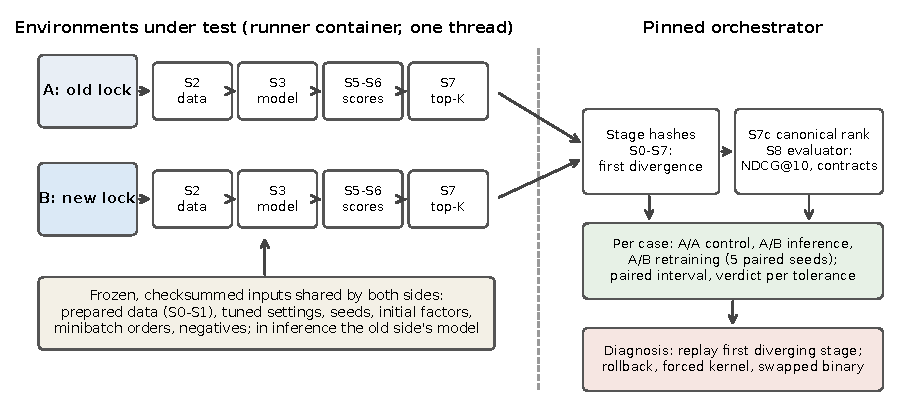
\includegraphics[width=\textwidth]{figures/study_design.pdf}
  \caption{Study design. Code under test imports only the standard library,
    NumPy, SciPy and the library under test, and exchanges arrays and JSON with
    the orchestrator, so an upgraded metric cannot masquerade as a changed
    recommender.}
  \label{fig:design}
\end{figure}

\subsection{Case selection}
We used a feasibility pilot as development evidence and froze the full-study
protocol and held-out manifests under the git tag \texttt{protocol-v1} before
building or running any held-out upgrade. The single-dependency collection
selects adjacent minor releases from PyPI metadata and takes the latest patch
of each minor within the January 2024--October 2026 window, for NumPy, SciPy
and pandas. The PyTorch manifest covers 2.9 to 2.15 only; we do not claim
exhaustive PyTorch coverage of the whole window. One direct requirement
changes per transition (Table~\ref{tab:transitions} in the appendix).

The snapshot collection resolves the unpinned requirements NumPy, SciPy,
pandas and \texttt{implicit} at quarterly upload cutoffs, at midnight UTC,
from 1~January 2024 through 1~October 2026 (Figure~\ref{fig:timeline}).
Those cutoffs limit the versions the resolver can see. Adjacent quarterly
snapshots form held-out bundle transitions. B1 is a separate development
bundle with a newer resolution cutoff of 1~November 2026. Identical resolved locks would remain in
the denominator as no-change transitions. In total the ledger holds
\nTransitions{} transitions: 23 single-dependency and 12 snapshot transitions,
of which 10 are development and 25 held-out.

A declared (transition, pipeline) case is applicable only if the pipeline
calls the changed package: a tracer counts calls into the relevant functions of the
upgraded package during a run, and pairs without such calls are recorded as
not applicable with that evidence. We tabulate the single-dependency and
snapshot collections, and the development and held-out splits, separately.
Twenty-nine issue-guided leads, mined from issue trackers and release notes,
were investigated for mechanisms and contribute no observations to the
systematic frequencies.

\begin{figure}[htbp]
  \centering
  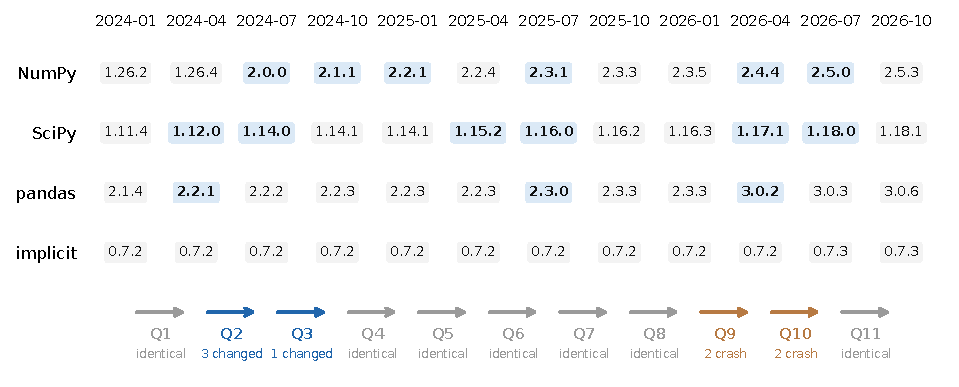
\includegraphics[width=\textwidth]{figures/snapshot_timeline.pdf}
  \caption{What an unpinned project would have installed at each quarterly
    cutoff, and the outcome of the six cases of each bundle transition on the
    primary host. Bold versions mark a new minor release. Q2 crosses NumPy~2.0
    and Q3 crosses NumPy~2.1; in Q9 and Q10 \texttt{implicit}~0.7.2 meets
    NumPy~2.4.}
  \label{fig:timeline}
\end{figure}

\subsection{Environments}
Each side of a transition is a locked environment, built with uv inside a
Linux runner container pinned by image digest, on Python~3.12, the only
interpreter that spans NumPy 1.26 to 2.5. Paired runs use the same host and
runner image, and one thread for BLAS, OpenMP and the model. The complete
lock diff defines the treatment, including any transitive differences. We
hold application source fixed across sides and screen resolution, build and
import before execution. For every environment we record the interpreter,
image, host, NumPy runtime information (SIMD features and BLAS), thread-pool
information and lockfile identity. Upstream test-suite screening is recorded
for the primary-host environments only.

\subsection{Data}
The primary dataset is MovieLens~1M \citep{grouplensmovielens,harper2015movielens}.
We verify the source archive by checksum and freeze the prepared interactions
and training-derived ID maps. For duplicate user--item events we retain the
earliest observation, using source order to break timestamp ties. We use a
global chronological split with nominal training, validation and test shares
of 76/10/14 (Table~\ref{tab:data}). A boundary timestamp belongs to the later
interval in its entirety. We selected these cutoffs using dataset counts
before running a recommender. A separate sensitivity analysis uses a nominal
per-user chronological 70/10/20 split.

An observed rating of at least~4 provides binary relevance. Evaluation
includes users observed in training who have at least one eligible relevant
item. The candidate catalogue comprises all 3{,}655 training items. We exclude
items the user interacted with during training for validation, and during
training or validation for testing, at any rating. Dataset files stay local
under the GroupLens research-use terms.

\begin{table}[htbp]
  \centering\small
  \caption{MovieLens~1M data accounting from the prepared-data manifest.
    Warm events have both IDs in the training mappings. Warm-relevant users
    are the eligible validation and test populations.}
  \label{tab:data}
  \begin{tabular}{@{}lrrrr@{}}
    \toprule
    Split & Raw events & Warm events & Warm users & Warm-relevant users \\
    \midrule
    \tablebody{tab_data_counts}
    \bottomrule
  \end{tabular}
\end{table}

As a declared scale check, we prepared MovieLens~20M with the same rules
under the tag \texttt{dataset-ml20m-v1}, before any run on it. Ratings are
floored to integers, and a fixed random sample of 2{,}000 warm relevant test
users (and 2{,}000 validation users) forms the evaluation population. Results on
MovieLens~20M are reported separately and never pooled with MovieLens~1M.

\subsection{Pipelines and models}
\label{sec:models}
Table~\ref{tab:pipelines} lists the eleven pipeline configurations. Let
$X\in\{0,1\}^{|U|\times|I|}$ hold the positive training interactions
(rating at least~4), with rows $x_u$.

\paragraph{Item-kNN (P1, and P2 cosine).} With item popularity
$n_i=\sum_u X_{ui}$, the reference pipeline \citep{sarwar2001itembased}
computes cosine similarities, keeps the $k$ most similar neighbours of each
item and scores by summation:
\begin{equation}
 s_{ij}=\frac{(X\T X)_{ij}}{\sqrt{n_i n_j}},\qquad
 N_k(i)=\topk_k\{s_{ij}: j\neq i\},\qquad
 z_u(i)=\sum_{j\in N_k(i)} X_{uj}\,s_{ij}.
 \label{eq:knn}
\end{equation}
Both $\topk_k$ in Equation~\eqref{eq:knn} and the final top-$K$ selection use
NumPy's \texttt{argpartition} followed by \texttt{argsort}. The pipeline runs
in float32 and in float64.

\paragraph{BM25 item-kNN (P2).} \texttt{implicit} re-weights the interaction
matrix before the cosine step \citep{robertson2009bm25}. With $m_i$
interactions of item $i$, mean $\bar m$, $n_u$ interactions of user $u$,
$K_1=100$ and $B=0.8$,
\begin{equation}
 w_{ui}=X_{ui}\,\frac{K_1+1}{K_1\,\ell_i+X_{ui}}\,
        \bigl(\ln|I|-\operatorname{log1p}(n_u)\bigr),\qquad
 \ell_i=(1-B)+B\,\frac{m_i}{\bar m}.
 \label{eq:bm25}
\end{equation}

\paragraph{Implicit ALS (P2).} ALS fits user and item factors $p_u,q_i\in
\mathbb{R}^d$ to the weighted least-squares objective of
\citet{hu2008implicit},
\begin{equation}
 \min_{P,Q}\ \sum_{u,i} c_{ui}\,\bigl(X_{ui}-p_u\T q_i\bigr)^2
 +\lambda\Bigl(\sum_u\|p_u\|^2+\sum_i\|q_i\|^2\Bigr),
 \label{eq:als}
\end{equation}
with confidence weights $c_{ui}$ scaled by $\alpha=20$, $\lambda=0.01$ and 15
alternating sweeps from frozen initial factors. Scores are $z_u(i)=p_u\T q_i$.

\paragraph{EASE (P6).} EASE \citep{steck2019ease} has the closed form
\begin{equation}
 P=(X\T X+\lambda I)^{-1},\qquad
 B_{ij}=\begin{cases}0,& i=j,\\ -P_{ij}/P_{jj},& i\neq j,\end{cases}\qquad
 Z=XB,
 \label{eq:ease}
\end{equation}
and Cornac computes $P$ with \texttt{numpy.linalg.inv}, that is, with the
LAPACK routines of the BLAS library bundled in the NumPy wheel.

\paragraph{SVD, SAR and ItemKNN (P3, P4, P6).} Surprise SVD predicts
$\hat r_{ui}=\mu+b_u+b_i+q_i\T p_u$ and is trained by stochastic gradient
descent. Recommenders SAR scores by item co-occurrence similarity (Jaccard,
cosine or lift) weighted by user affinity. Cornac ItemKNN is a second,
independent item-neighbourhood implementation.

\paragraph{BPR (P7).} The reference BPR model \citep{rendle2009bpr} has
float32 embeddings $p_u,q_i$, score $p_u\T q_i$ and the loss
\begin{equation}
 \mathcal{L}=-\frac{1}{|\mathcal B|}\sum_{(u,i^+,i^-)\in\mathcal B}
 \ln\sigma\bigl(p_u\T q_{i^+}-p_u\T q_{i^-}\bigr)
 +10^{-4}\,\overline{\|p_u\|^2+\|q_{i^+}\|^2+\|q_{i^-}\|^2},
 \label{eq:bpr}
\end{equation}
optimised with Adam (learning rate 0.01, 10 epochs, batches of 4{,}096). The
initial embeddings, the minibatch order and the negative items are generated
once in the orchestrator and loaded on both sides, so that only PyTorch's
arithmetic and \texttt{torch.topk} can differ. P7 runs on CPU and, as a
separate condition, on a GPU. RecBole is not included. Upstream reports
describe a crash under NumPy~2 from the removed \texttt{np.bool8} alias
(Table~\ref{tab:leads}); we did not run it ourselves.

Each configuration is declared before its ranking runs. We select the
hyperparameter by baseline validation NDCG@10 with a fixed grid order for
ties, then carry the selected setting to both test environments. Every
pipeline selected the same value in every baseline environment
(Table~\ref{tab:pipelines}). The validation NDCG@10 of a grid value differed
between baseline environments by at most \tuningSpread{}, which is less than
the smallest gap between a selected value and the runner-up (\tuningGap{}).

\begin{table}[htbp]
  \centering
  \caption{Pipeline configurations. Tuned and Grid: the tuned hyperparameter
    and its values. Selected: the value chosen on baseline validation data,
    verified against the run metadata for both sides of each successful
    comparison. Parentheses count cases with verified selections. Cases
    counts all primary MovieLens~1M cases in the configuration. The
    supplement records validation candidates, scores and run IDs.}
  \label{tab:pipelines}
  \scriptsize\setlength{\tabcolsep}{2pt}
  \begin{tabular}{@{}lllllllr@{}}
    \toprule
    ID & Library & Model & dtype & Tuned & Grid & Selected (cases) & Cases \\
    \midrule
    \tablebody{tab_x_pipelines}
    \bottomrule
  \end{tabular}
\end{table}

\subsection{Hosts and devices}
All primary runs used one host (A, AMD Ryzen~7 7840HS, Zen~4, with AVX-512 and
BF16). Declared subsets were repeated on rented hosts: B, an AMD EPYC 7R13
(Zen~3, AVX2 only, \nHostB{} cases); C, an Intel Xeon Platinum 8259CL
(Cascade Lake, AVX-512 without BF16, \nHostC{} cases); and an NVIDIA Tesla T4
GPU for the PyTorch cases (\nHostGpu{} cases). Each host has its own ledger,
and comparisons never mix hosts. Each host's case set was declared before
it ran. The rented-host case sets were later run a second time with all raw
arrays retained (Table~\ref{tab:reruns}). The NumPy wheel bundles its own OpenBLAS, which chooses a kernel family
at import time from the processor's features. Table~\ref{tab:blas} records what
each NumPy wheel bundled and selected on each host.

\begin{table}[htbp]
  \centering\small
  \caption{OpenBLAS release family bundled in the NumPy wheel and the kernel family it
    selected at run time on each CPU host, as recorded by the environment
    probe. For each NumPy version, the same wheel is installed on every host.
    The displayed release family omits build suffixes.}
  \label{tab:blas}
  \begin{tabular}{@{}llccc@{}}
    \toprule
    NumPy & Bundled OpenBLAS & Host A (Zen~4) & Host B (Zen~3) & Host C (Cascade Lake) \\
    \midrule
    \tablebody{tab_x_blas}
    \bottomrule
  \end{tabular}
\end{table}

\subsection{Controls}
For ranking cases, we run a same-environment A/A inference comparison
before comparing versions. The control must reproduce the stage artifacts
bit for bit and yield zero metric differences. Preprocessing uses old and
new environments without a separate A/A run. In A/B inference, the two sides
use the same checksum-verified portable model arrays and fixed candidates.
Retraining holds the data, input order and settings fixed, with five paired
seeds and shared random artifacts, such as initial factors, minibatch orders
and negative samples, generated once in the orchestrator where the adapter
supports them.

\subsection{Outcomes}
The native ordering supplies the primary quality result. The diagnostic
canonical ordering sorts all eligible scores in descending order and breaks
exact ties by ascending external item ID, including the entire tie block at
the cutoff before selection (Section~\ref{sec:ties}). We record top-10 set
overlap, changed lists, shared-item position changes and exact cutoff ties.
We require unique, valid and unseen items, finite scores, and a list length
equal to the smaller of the cutoff and the eligible count. A contract
violation takes precedence over a quality verdict.

Binary NDCG@10 is primary (Equation~\ref{eq:ndcg}); Recall@10 and NDCG@20 are
secondary. Stage digests locate the first divergence
(Equation~\ref{eq:first-divergence}, Table~\ref{tab:stages}). For attributed
mechanisms we replay the implicated stage on frozen upstream inputs and use
rollback, repair, forced library behaviour or reapplication.

\begin{table}[htbp]
  \centering\small
  \caption{Checkpoints. The canonical ranker and the evaluator run outside
    the environment under test.}
  \label{tab:stages}
  \begin{tabularx}{\textwidth}{@{}llX@{}}
    \toprule
    Stage & Object & Diagnostic role \\
    \midrule
    S0--S2 & Inputs, ID maps, interactions & Establish identical data and preprocessing. \\
    S3 & Fitted parameters & Identify training or model-construction differences. \\
    S4 & Candidate IDs & Distinguish candidate membership from score ordering. \\
    S5--S6 & Scores and seen mask & Separate numerical variation from eligibility changes. \\
    S7 & Native top-$K$ & Record the order returned by the implementation. \\
    S7c & Canonical top-$K$ & Diagnose exact ties with score and item-ID ordering. \\
    S8 & Quality and contracts & Evaluate relevance and admissibility independently. \\
    \bottomrule
  \end{tabularx}
\end{table}

\subsection{Statistics}
Loss is baseline minus upgraded NDCG@10, so positive values are losses
(Equation~\ref{eq:loss}). We weight eligible users and seed pairs equally. For
deterministic inference, the interval is the percentile interval of
$B=10{,}000$ paired-user bootstrap resamples,
\begin{equation}
 I=\bigl[\widehat L^{*}_{(\alpha/2)},\ \widehat L^{*}_{(1-\alpha/2)}\bigr],\qquad
 \widehat L^{*b}=\frac{1}{|U|}\sum_{j=1}^{|U|} d_{u^b_j},\quad
 u^b_j\sim\mathrm{Unif}(U),\quad \alpha=0.05,
 \label{eq:bootstrap}
\end{equation}
with a fixed analysis seed. Retraining uses the paired $t$ interval on the
five seed-level mean losses (Equation~\ref{eq:interval}), conditional on the
fixed evaluation users and split. A zero-width retraining interval means the
seed-level mean losses coincide. The inference bootstrap measures variation
under resampling of evaluation users. A sensitivity interval resamples paired
seeds and then users. Protocol~v1 prescribes a rerun
with ten additional fixed seeds if the primary retraining interval is
inconclusive at $\delta=0.005$; no case required it.

We report verdicts at the absolute NDCG tolerances
$\delta\in\{0.002,0.005,0.010\}$ with the rule of Equation~\eqref{eq:verdict}.
These margins express absolute differences on the NDCG scale. Their
percentage sizes relative to observed baseline quality appear in
Table~\ref{tab:baseline}; the study does not calibrate them to production
outcomes. Equivalence requires interval containment. For the paired $t$
interval, the corresponding two one-sided tests use level 0.025 each
\citep{schuirmann1987tost}. The percentile bootstrap uses the containment
rule directly. We form low, medium and high activity groups using the nearest-rank
training-count tertiles. The primary split contains 223, 277 and 507 eligible
test users in the three groups. Within a case and mode, each group interval
uses a Bonferroni-adjusted level of $1-0.05/3$.

\subsection{Synthetic positive controls}
\label{sec:synthetic-design}
Because no real case showed harm, RQ3 uses synthetic faults applied to the
new side's saved inference outputs of the \synBase{} held-out MovieLens~1M
ranking cases that have an accepted A/A control and a completed A/B
comparison. The faults were declared with the probe policy before any was
generated: F1 swaps the identifiers of 1\% of items (37 of 3{,}655 score
columns are rotated), F2 drops the seen-item mask, F3 rounds scores to two
decimals, and F4 reverses the ranking of 1\% of users (11 of 1{,}007). The
full-population evaluator labels each faulted output, and an output counts as
a \emph{positive} at tolerance $\delta$ if it is a contract failure or harmful
at $\delta$.

\paragraph{Fault isolation (analysis version 2).} The first implementation
rebuilt every user's list with a reference ranker, which let reconstruction
effects leak into users outside a fault's scope; an evidence audit found this
after the first analysis. The reported analysis is a corrected, versioned
rerun; the first analysis is retained unchanged in the study records, and the
cohort, fault definitions, random selections, detectors and primary
configuration are the same. Let $\rho$ be a reference ranker,
$(z_u,m_u)$ the saved scores and seen mask of user $u$, $(z'_u,m'_u)$ their
faulted versions and $\pi^B_u$ the saved native list. The faulted list is
\begin{equation}
 \pi'_u=\begin{cases}
   \pi^B_u, & \rho(z'_u,m'_u)=\rho(z_u,m_u),\\
   \rho(z'_u,m'_u), & \text{otherwise,}
 \end{cases}
 \label{eq:isolation}
\end{equation}
so a list changes only where the fault changes the reference ranking. For F1
and F2, $\rho$ orders by descending score and resolves exact ties in the saved
native order, so that $\rho(z_u,m_u)$ reproduces the native list and the
reconstruction adds no tie reordering of its own; it reproduced the native
top-10 list of every user in every base case. For F3, which creates ties by
rounding, $\rho$ is the pipeline-independent \texttt{argpartition} ranker,
whose handling of those ties is part of the fault. F4 replaces exactly the
reversed rows. A no-fault control, F0, applies the full pipeline-independent
rebuild without any fault and measures what reconstruction alone does.

\paragraph{Detectors.} Probe panels contain 100, 300 or 1{,}000 of the 1{,}007
users, drawn uniformly, proportionally by activity stratum, or by smallest
score margin at the cutoff; a panel raises an alarm if the verdict rule applied
to its users is harmful or a contract failure. The baselines are exact snapshot
(any native top-10 list differs), score tolerance (eligible scores are
non-finite, or their relative $L_2$ difference is undefined or exceeds
$10^{-6}$), list overlap (strict: any top-10 set
changes; lenient: mean overlap below 0.99) and the full labelled check. False
alarms are counted on real A/A pairs and on real A/B pairs whose verdict is
equivalent, which represent benign upgrade churn. The primary detector
(activity strata, 300 users, $\delta=0.005$) was named before the first
evaluation.

For eligible baseline scores sorted in descending order, the margin selector
uses the normalised gap
\begin{equation}
 m_u=\frac{z^A_{u,(K)}-z^A_{u,(K+1)}}
              {\max_{i\in C_u}z^A_u(i)-\min_{i\in C_u}z^A_u(i)}.
 \label{eq:margin}
\end{equation}
Constant-score rows receive margin zero; rows with at most $K$ eligible items
have an undefined margin and sort after defined rows. A fixed seeded random
priority breaks equal margins. The request proxy and the recall are
\begin{equation}
 C_{\mathrm{requests}}(P)=2|P|,\qquad
 \operatorname{Recall}(P)=\frac{\sum_{j\in\mathcal H}a_P(j)}{|\mathcal H|},
 \label{eq:recall}
\end{equation}
where $a_P(j)$ is the recorded alarm and $\mathcal H$ contains the synthetic
positives. The evaluation reuses saved scores, and the margin selector needs
baseline scores for all users, so $C_{\mathrm{requests}}$ is a proxy and not a
measured cost.

% ---------------------------------------------------------------------------
\section{Results}
\label{sec:results}

\subsection{RQ1: Outcomes of eligible upgrades}

On the primary host, \nEnvsOk{} of \nEnvs{} environments built and imported. The
\nEnvsResolveFailed{} that did not resolve were genuine conflicts: Recommenders
requires \texttt{pandas<3}, and Cornac~3.1 requires NumPy~$>2.0$. Together they
exclude eight declared transition--pipeline cells (hatched in
Figure~\ref{fig:matrix}). The ledger records \nRunsOk{} completed runs,
\nRunsCrash{} crashes and \nRunsTimeout{} timeout\footnote{A development run
that timed out after the host slept; the case was rerun and the timeout
remains in the ledger.}, \computeHours{} hours of run time in total
(Table~\ref{tab:cost}).

Figure~\ref{fig:matrix} shows every primary case, and Table~\ref{tab:rq1}
counts them. \nIdentical{} cases produced identical checkpoints on both sides,
\nChanged{} changed a checkpoint silently, \nFailure{} failed visibly and
\nNotApplicable{} were not applicable. Of the \nChanged{} changed cases,
\nListChanged{} changed a top-10 list and \nCheckpointOnly{} changed only
earlier checkpoints. No completed ranking comparison showed a supported
quality regression, a contract violation or an inconclusive verdict at any of
the three tolerances. Runtime failures and inapplicable configurations have no
quality verdict. The \nChanged{} changed cases are spread across
\nTransitionsChanged{} of \nTransitions{} transitions. Each transition can
affect several pipelines, and some transitions carry the same upstream change.
The relative size of a fixed margin varies by pipeline
(Table~\ref{tab:baseline}): for most it is 1\% to 2\% of the baseline at the
smallest margin, but Cornac ItemKNN is a weak configuration here (NDCG@10 of
0.039), and the same margin is 5\% of its quality.

\begin{table}[htbp]
  \centering
  \caption{Baseline test NDCG@10 for completed primary ranking comparisons.
    Ranges are over cases, using one frozen model in inference and averaging
    the baseline seed means in retraining. The final three columns express
    each absolute margin as a percentage of the baseline.}
  \label{tab:baseline}
  \small
  \begin{tabular}{@{}llrrrrr@{}}
    \toprule
    Pipeline & Mode & Cases & Baseline NDCG@10 & 0.002 & 0.005 & 0.010 \\
    \midrule
    \tablebody{tab_x_baseline}
    \bottomrule
  \end{tabular}
\end{table}

\begin{figure}[htbp]
  \centering
  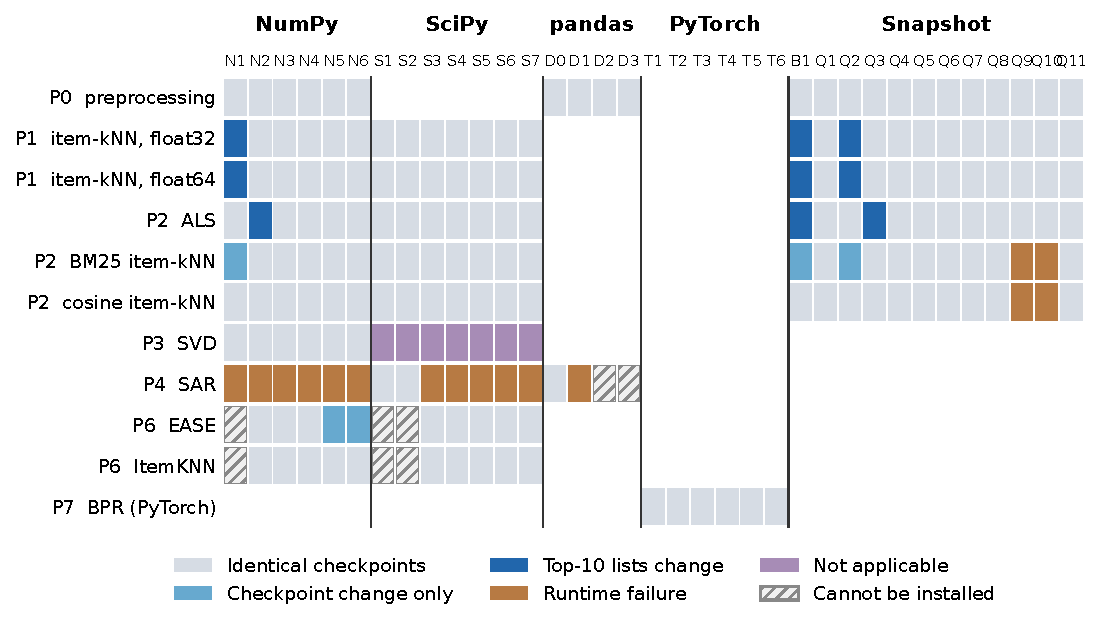
\includegraphics[width=\textwidth]{figures/case_matrix.pdf}
  \caption{All \nCases{} primary cases: one cell per transition and pipeline
    configuration on MovieLens~1M, host A. Empty cells are not declared cases.
    Transition labels in brown are development cases; the others are held-out.
    B1 is the development snapshot bundle (June 2024 to November 2026).}
  \label{fig:matrix}
\end{figure}

\begin{table}[htbp]
  \centering
  \caption{Outcomes per case on MovieLens~1M, primary host. A case is
    \emph{changed} if any checkpoint differs between sides, in inference or
    retraining, and its quality verdict is equivalent at all three tolerances.
    \emph{Failure} counts case-level execution failures. The eight cells that
    could not be installed, the N1 sensitivity split and MovieLens~20M are
    reported separately.}
  \label{tab:rq1}
  \footnotesize\setlength{\tabcolsep}{3pt}
  \begin{tabular}{@{}llrrrrrrrr@{}}
    \toprule
    Collection & Split & Cases & Ident. & Changed & Regr. & Contr. & Unc. & Failure & N/A \\
    \midrule
    \tablebody{tab_rq1}
    \bottomrule
  \end{tabular}
\end{table}

\begin{table}[htbp]
  \centering
  \caption{Outcomes per pipeline configuration on MovieLens~1M, primary host.
    Model: a checkpoint changes but no top-10 list. Lists: a top-10 list
    changes. Excluded: declared cells whose environment does not resolve.}
  \label{tab:pipeline-outcomes}
  \footnotesize\setlength{\tabcolsep}{4pt}
  \begin{tabular}{@{}llrrrrrrr@{}}
    \toprule
    ID & Pipeline & Cases & Identical & Model & Lists & Failure & N/A & Excluded \\
    \midrule
    \tablebody{tab_x_pipeline_outcomes}
    \bottomrule
  \end{tabular}
\end{table}

\paragraph{Visible failures.} The \nFailure{} crashes come from two
downstream incompatibilities, and a third prevents installation
(Table~\ref{tab:mechanisms}). Recommenders~1.2.1 SAR uses the \texttt{np.NaN}
alias removed in NumPy~2.0 and crashes in every NumPy~2 environment
(\nCasesMechSix{} cases). In the snapshot of 1~April 2026, an unpinned project
resolved \texttt{implicit}~0.7.2 next to NumPy~2.4.4, and its item-kNN models
crash on the missing \texttt{np.in1d} (\nCasesMechSeven{} cases, Q9 and Q10 in
Figure~\ref{fig:timeline}); the snapshot of 1~July, with
\texttt{implicit}~0.7.3, runs. Recommenders cannot be installed next to
pandas~3. These failures are visible to any execution check.

\paragraph{Preprocessing, SciPy, pandas and PyTorch.} All 22 preprocessing
comparisons, including the snapshots spanning pandas 2.3 to 3.0, kept
identical checkpoints. No SciPy, pandas or CPU PyTorch transition changed a
checkpoint in a comparison that completed. Every silent change on the primary
host involves a NumPy transition or a snapshot that contains one
(Figure~\ref{fig:matrix}).

\paragraph{Precision of the comparisons.} The \nCompleted{} completed cases
contain \nCaseModes{} ranking comparisons (inference and retraining of 156
ranking cases). In \nDegenerate{} of them every user had the same NDCG@10 on
both sides, so the interval is exactly $[0,0]$. The remaining
\nNonDegenerate{} are the ALS retraining comparisons, whose interval
half-width is at most \maxHalfWidth{}, about one ninth of the smallest
tolerance. Across the primary ranking comparisons the largest absolute interval bound is
\worstNdcgTen{} for NDCG@10, \worstRecallTen{} for Recall@10 and
\worstNdcgTwenty{} for NDCG@20. The equivalence verdicts therefore do not rest
on wide intervals.

\paragraph{Other hosts, devices and data.}
All \nHostB{} cases on host B, \nHostC{} on host C and \nHostGpu{} on the GPU
were equivalent at every tolerance. On MovieLens~20M, all \nMLtwentyCases{}
declared cases were equivalent and \nMLtwentyChanged{} changed a checkpoint.
The largest point loss across the real comparisons, \lossMOneMLtwenty{}
NDCG@10, came from tie reordering on MovieLens~20M and is about one eighteenth
of the smallest tolerance. Table~\ref{tab:extensions} in the appendix lists the
scale and split-sensitivity results, and Figure~\ref{fig:churn-quality} places
them beside the primary observations without pooling their populations.

\paragraph{Reproduction of the rented-host results.}
The first Jobs on the rented hosts exported reports and metadata but not their
arrays. We therefore ran the three case sets a second time, as declared
additions to the frozen results, with the fitted model, scores and ranked
lists of every run exported and checksummed (Table~\ref{tab:reruns}). The
second Jobs ran on the same CPU models as the first. All \rerunRuns{} runs
reproduced the stage digests of their counterparts in the first Jobs
(\rerunHashesEqual{} of \rerunHashes{} digests equal), and all \rerunCases{}
cases had the same outcome. The pinned local evaluator, run on the downloaded
arrays, reproduced the per-user metrics that the Jobs had written for all
\rerunEvaluated{} runs. The reproduction includes the GPU training difference
M5: the changed model is itself stable from one Job to the next.

\begin{table}[htbp]
  \centering
  \caption{Second run of the rented-host case sets with raw arrays retained.
    Digests: stage digests S0--S8 equal to the first Job's, of those compared.
    Outcome: cases with the same comparison outcome as in the first Job.
    Files: files in the downloaded archives that match their recorded
    SHA-256. Re-evaluated: runs whose per-user metrics, recomputed locally
    from the arrays, equal the Job's.}
  \label{tab:reruns}
  \footnotesize\setlength{\tabcolsep}{4pt}
  \begin{tabular}{@{}lrrrrrrr@{}}
    \toprule
    Host & Cases & Runs & Digests & Outcome & Archive (GB) & Files & Re-evaluated \\
    \midrule
    \tablebody{tab_x_reruns}
    \bottomrule
  \end{tabular}
\end{table}

\begin{figure}[htbp]
  \centering
  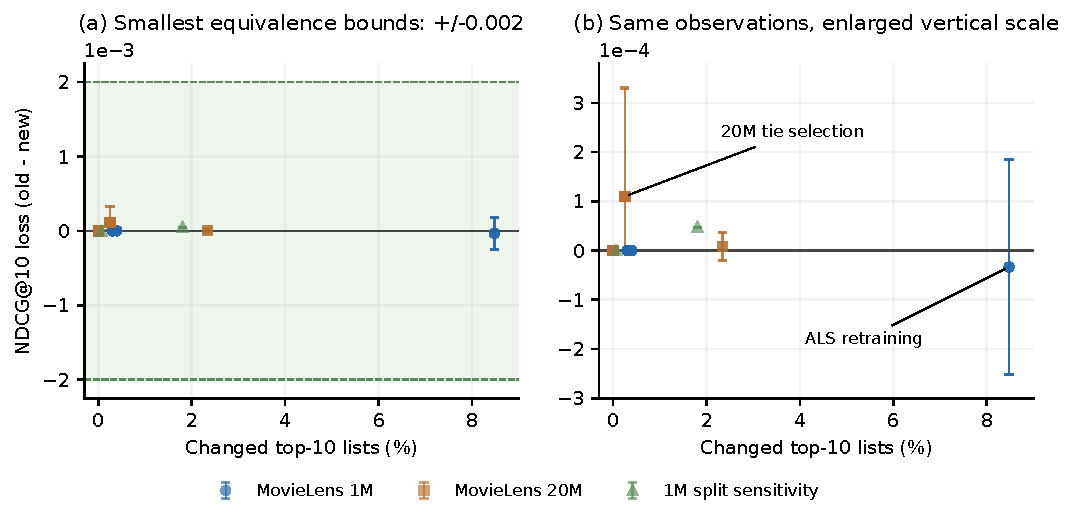
\includegraphics[width=\textwidth]{figures/churn_quality.pdf}
  \caption{List churn versus offline quality loss for the completed
    primary-host comparisons, with the scale and split-sensitivity extensions
    distinguished. Inference intervals bootstrap users; retraining intervals
    use paired seed means. Left: against the smallest equivalence bounds.
    Right: the same observations at a finer vertical scale. These are
    within-case intervals, not a prevalence estimate or a fitted relationship
    between churn and harm.}
  \label{fig:churn-quality}
\end{figure}

\paragraph{Upstream test suites.} Table~\ref{tab:suites} reports the status
of each library's own test suite in the screened environments. Only
\texttt{implicit}~0.7.3 (155 tests) and part of the NumPy suites ran to a clean
pass. NumPy's suite passed in 29 environments; in 46 it was recorded as failed
with between 1 and 9 failing tests among more than 37{,}000, and Surprise
recorded the same 59 failures in every environment.
The failures we inspected come from the minimal test harness (fixture files
that the Surprise source distribution does not ship, and build tooling for
NumPy's \texttt{f2py} and limited-API tests), not from numerical tests. SciPy,
pandas, Recommenders and PyTorch suites did not complete within the time cap.
In our harness, then, the upstream suites could not act as a gate for the
changes reported below. This describes how far the suites could be run here,
not their content.

\begin{table}[htbp]
  \centering\small
  \caption{Upstream test-suite status per environment on the primary host
    (number of environments). Unavailable: the installed artifact ships no
    tests. Not runnable: the suite did not complete within the time cap or
    lacked required tooling.}
  \label{tab:suites}
  \begin{tabular}{@{}lrrrr@{}}
    \toprule
    Package & Passed & Failed & Unavailable & Not runnable \\
    \midrule
    \tablebody{tab_x_suites}
    \bottomrule
  \end{tabular}
\end{table}

\paragraph{Answer to RQ1.} A checkpoint changed silently in \nChanged{} of
\nCases{} cases (\nDevChanged{} development, \nHeldoutChanged{} held-out), and
a top-10 list in \nListChanged{}. None reached a supported offline quality loss
or a contract violation. The outcomes that would stop a project were visible
failures: \nFailure{} crashes and eight uninstallable cells.

\subsection{RQ2: Affected stages, users and mechanisms}

Table~\ref{tab:changed} lists every changed case and mode with its quality
result, and Table~\ref{tab:numeric} gives the size of the numerical difference.
In inference, where both sides load the same model, changes appear only at
native top-$K$ selection (S7), with identical scores. In retraining, every
change first appears in the fitted model (S3). The largest mean fraction of
changed top-10 lists is 8.48\%, averaged over paired seeds. Every primary
loss interval is contained in $[-\delta,\delta]$ for the smallest tolerance,
and the widest activity-group interval bound is \groupBound{}, so no activity
group carries a supported material loss at the declared tolerances
(Figure~\ref{fig:groups}). This does not exclude smaller group effects.

\begin{table}[htbp]
  \centering
  \caption{Every changed case and mode on MovieLens~1M (primary host). Stage:
    first differing checkpoint. Users: percentage of test users whose native
    top-10 list changed, averaged across paired seeds for retraining.
    Loss: NDCG@10, baseline minus upgraded, with its 95\%
    interval. Group: largest absolute bound of the three activity-group
    intervals (Bonferroni-adjusted). B1 and Q2 contain NumPy 1.26 to 2.0; B1
    and Q3 contain NumPy 2.0 to 2.1.}
  \label{tab:changed}
  \footnotesize\setlength{\tabcolsep}{3pt}
  \begin{tabular}{@{}lllcrlr@{}}
    \toprule
    Case & Split & Mode & Stage & Users\,\% & Loss [95\% interval] & Group \\
    \midrule
    \tablebody{tab_changed}
    \bottomrule
  \end{tabular}
\end{table}

\begin{table}[htbp]
  \centering
  \caption{Numerical size of every changed comparison in Table~\ref{tab:changed}.
    Max: largest absolute difference of an eligible score between sides.
    Rel.: relative $L_2$ difference of the eligible scores (zero where it
    underflows against the largest scores). Overlap: mean top-10 set overlap
    (Equation~\ref{eq:overlap}). Moved: percentage of shared top-10 items
    that changed position. Canon.: whether the canonical rankings are equal.}
  \label{tab:numeric}
  \footnotesize\setlength{\tabcolsep}{3pt}
  \begin{tabular}{@{}lllrrrrrc@{}}
    \toprule
    Case & Mode & Mech. & Max & Rel. & Users\,\% & Overlap & Moved\,\% & Canon. \\
    \midrule
    \tablebody{tab_x_numeric}
    \bottomrule
  \end{tabular}
\end{table}

\begin{figure}[htbp]
  \centering
  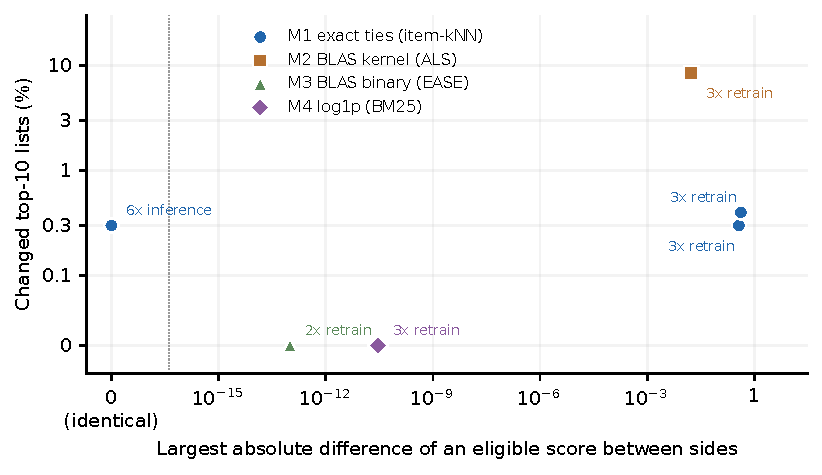
\includegraphics[width=.86\textwidth]{figures/perturbation_churn.pdf}
  \caption{Size of the score difference against list churn for the changed
    comparisons of Table~\ref{tab:numeric}; labels count coinciding
    comparisons. The size of a numerical difference does not predict whether
    lists change: identical scores change lists through ties (M1, left),
    while differences of $10^{-13}$ to $10^{-11}$ change none (M3, M4).}
  \label{fig:perturbation}
\end{figure}

Figure~\ref{fig:perturbation} shows why a score-difference threshold is a poor
proxy for ranking change. The comparisons with the largest list churn after
ALS have score differences near $10^{-2}$, the tie comparisons change lists
with a score difference of exactly zero, and the last-bit comparisons change
models and scores without touching a list.

Table~\ref{tab:mechanisms} groups the changed and failed cases by mechanism.
A mechanism is the unit of independence: the same upstream change reappears in
the single-dependency and snapshot cases that contain it, and the snapshot
cases reproduce their single-dependency counterparts exactly, down to the
fitted model for ALS. Section~\ref{sec:mechanisms} describes each mechanism and
how it was attributed.

\begin{table}[htbp]
  \centering
  \caption{Mechanisms and incompatibilities. Primary counts cover MovieLens~1M
    on host A. Extension counts cover the alternate split, MovieLens~20M
    replays and GPU, with the additional CPU replays reported separately.
    Effects use primary comparisons for M1--M4 and the GPU comparison for M5.
    M8 counts two excluded SAR cells outside the primary denominator.}
  \label{tab:mechanisms}
  \small
  \begin{tabularx}{\textwidth}{@{}l>{\raggedright\arraybackslash}Xrrll@{}}
    \toprule
    & Mechanism & Primary & Extension & Stage & Effect \\
    \midrule
    \tablebody{tab_mechanisms}
    \bottomrule
  \end{tabularx}
\end{table}

\begin{figure}[htbp]
  \centering
  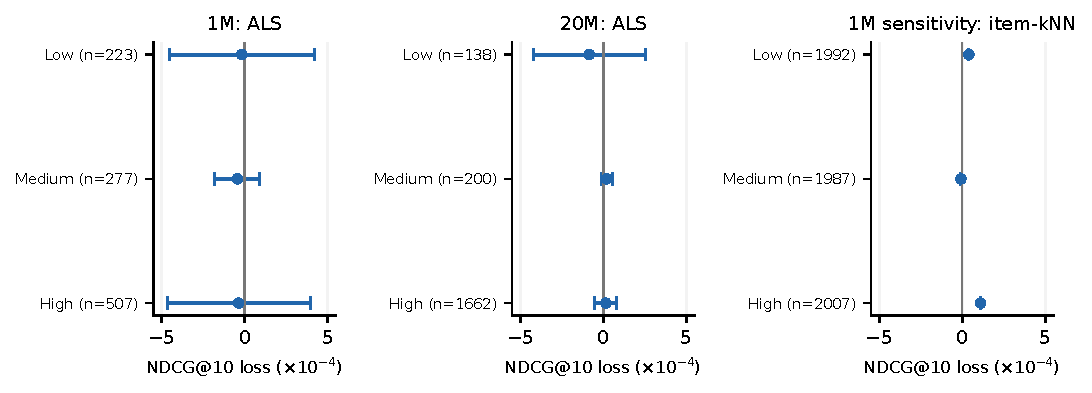
\includegraphics[width=\textwidth]{figures/activity_intervals.pdf}
  \caption{Retraining losses by predeclared activity group for ALS on each
    dataset and for reference item-kNN on the separate per-user split.
    Intervals use paired seed means with Bonferroni adjustment within each
    case and mode. The displayed range is narrower than the smallest
    equivalence bounds ($\pm0.002$). Degenerate intervals reflect identical
    seed-level mean losses.}
  \label{fig:groups}
\end{figure}

\paragraph{Hardware dependence.} Figure~\ref{fig:blas} and
Table~\ref{tab:hardware} repeat the mechanism cases on the three CPUs. Only
M1, tie reordering, appears on every CPU. M2 appears only on host A, where
OpenBLAS switches from its Cooperlake to its SkylakeX kernels between
NumPy~2.0 and~2.1. Host B changes kernel family at the same NumPy release
(Zen to Haswell) without any change in results, and host C, lacking BF16,
uses SkylakeX for every NumPy version; its absence of change was predicted in
the host declaration before the run. On host A, the forced-core replay
reproduced the upgraded ALS output on the baseline environment. M3 and M4 appear on
both AVX-512 CPUs and not on the AVX2 CPU. Controls stayed identical on all
hosts. On the GPU, PyTorch 2.9.1 to 2.10.0 changed the trained BPR model (M5),
while all seven PyTorch versions trained bit-identical models on the CPUs.

\begin{figure}[htbp]
  \centering
  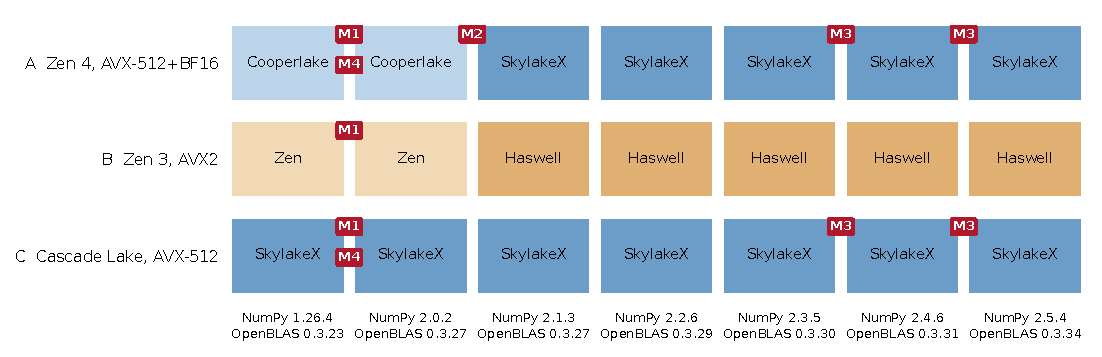
\includegraphics[width=\textwidth]{figures/blas_map.pdf}
  \caption{Kernel family selected by the bundled OpenBLAS for each NumPy wheel
    on the three CPU hosts (Table~\ref{tab:blas}). A red label between two
    wheels marks a mechanism whose case changed a checkpoint on that host for
    that NumPy transition. M1 and M4 belong to the NumPy~2.0 code itself and
    not to OpenBLAS; they are shown at the transition where they occur.}
  \label{fig:blas}
\end{figure}

\begin{table}[htbp]
  \centering
  \caption{Checkpoint change of the mechanism cases on three CPUs (inference
    or retraining). A: AMD Zen~4, AVX-512 with BF16. B: AMD Zen~3, AVX2.
    C: Intel Cascade Lake, AVX-512 without BF16. ctl: control cases selected
    to show no change.}
  \label{tab:hardware}
  \small
  \begin{tabular}{@{}llccc@{}}
    \toprule
    & Case & A & B & C \\
    \midrule
    \tablebody{tab_hardware}
    \bottomrule
  \end{tabular}
\end{table}

\paragraph{Answer to RQ2.} Silent changes enter at two stages: top-$K$
selection with exact ties, and fitted parameters during retraining. Four
attributed numerical mechanisms explain the primary changes, and the GPU adds
an unresolved one. M2--M5 vary with the tested host or device. The ALS
replay isolates a process-wide core setting, while the EASE replay isolates
the bundled OpenBLAS binary. No evaluated
activity group shows a supported material loss. Three CPUs do not establish
hardware independence for M1, and they do not isolate a single processor
feature for M2--M4.

\subsection{RQ3: Separating churn from harm}

\paragraph{What the faults do.} Table~\ref{tab:syn-labels} gives the
full-population label of every synthetic output and the footprint of each
fault. F2 violates the contract in all \synBase{} base cases. F3 violates it in
30: the \texttt{implicit} neighbourhood models mark unscorable items with the
most negative float, which \texttt{numpy.round} overflows to $-\infty$, and
the evaluator rejects non-finite scores. F1 is harmful in \synFOne{} base cases
at $\delta=0.005$ and inconclusive or equivalent in the rest. F4 changes
exactly \synFFourMaxUsers{} users and costs a median of \synFFourMedianLoss{}
NDCG@10 on the population; it is never labelled harmful, at any of the three
tolerances. In these cases the population-level rule did not label even
complete reversals for a small set of users as harmful. At $\delta=0.005$
there are \synPositives{} positives: \synQualityPositives{} quality positives
(all F1) and \synContractPositives{} contract positives.

The no-fault control shows why isolation matters. Rebuilding the lists with
the pipeline-independent ranker and no fault changed at least one list in
\synControlChangedCases{} of \synBase{} base cases, and up to
\synControlMaxUsers{} of 1{,}007 users, purely through tie order. The full
check labels none of these outputs harmful. An alternative valid tie order
can still change measured NDCG. The real benign controls comprise
\synBenign{} pairs, of which only \synSnapshotBenign{} changed under the
exact snapshot comparison, limiting what zero panel alarms establish.

\begin{table}[htbp]
  \centering
  \caption{Synthetic outputs at $\delta=0.005$: full-population reference
    labels over the \synBase{} base cases, and the footprint of each fault.
    Users: number of users whose native top-10 list differs from the saved
    one (median and maximum over base cases). Loss: median full-population
    NDCG@10 loss over the outputs without contract violations.}
  \label{tab:syn-labels}
  \footnotesize\setlength{\tabcolsep}{3pt}
  \begin{tabular}{@{}lrrrrrrr@{}}
    \toprule
    Fault & Contr. & Harmful & Inconcl. & Equiv. & Users med. & max. & Loss \\
    \midrule
    \tablebody{tab_x_syn_labels}
    \bottomrule
  \end{tabular}
\end{table}

\paragraph{Detection.} Table~\ref{tab:rq3} reports every detector. No detector
alarmed on a real A/A pair. All panels detect every contract positive, even
with 100 users, because a dropped mask or a non-finite score affects most
users. Quality positives are harder (Figure~\ref{fig:detection}a). The
pre-specified primary panel (activity strata, 300 users) detects
\synPrimaryFOne{} of \synFOne{} and has recall \synRecallPrimary{}; a uniform
panel of the same size does the same. A panel of 300 users with the smallest
score margin at the cutoff detects all \synFOne{} (recall
\synRecallMargin{}), as do all panels of 1{,}000 of the 1{,}007 eligible users.
No panel alarmed on a
real benign upgrade.

The change detectors trade one failure for another. Exact snapshot and strict
overlap detect every positive, but they also alarm on \synSnapshotBenign{} of
\synBenign{} real benign upgrades and on \synControlSnapshotAlarms{} of
\synBase{} no-fault controls. Tie handling can change item order, which
triggers the exact check, or membership, which triggers both checks. The score
tolerance misses every dropped mask (recall \synRecallScoreTol{}), because F2
does not change scores. The lenient overlap threshold misses every rounding
fault (recall \synRecallLenient{}).

The margin panel selects users near the ranking boundary. Its loss estimate
need not represent the population. Selection requires baseline scores for
all eligible users.
It alarmed on \synControlPanelAlarms{} of the \synBase{} no-fault
controls, the three Surprise SVD cases, where reordered ties change the lists
of 230 of 1{,}007 users at a population loss of 0.0033 and which the full
check labels inconclusive rather than harmful. A margin panel is therefore a sensitive
screen whose alarms need confirmation by the full check, not an unbiased
estimator.

\begin{table}[htbp]
  \centering
  \caption{Detection of synthetic positives at $\delta=0.005$ with isolated
    faults. F1--F3: detected positives per fault (F4 has no positive at this
    tolerance). A/A and Benign: alarms on real A/A pairs and on real benign
    A/B pairs. F0: alarms on the no-fault reconstruction control. Requests: a
    paired-user count proxy (two per user), excluding baseline panel selection
    and training. The full labelled check defines the reference positives,
    so its recall is one by construction.}
  \label{tab:rq3}
  \footnotesize\setlength{\tabcolsep}{3pt}
  \begin{tabular}{@{}lrrrrrrrrr@{}}
    \toprule
    Detector & Recall & F1 & F2 & F3 & F4 & A/A & Benign & F0 & Requests \\
    \midrule
    \tablebody{tab_x_syn_detect}
    \bottomrule
  \end{tabular}
\end{table}

\begin{figure}[htbp]
  \centering
  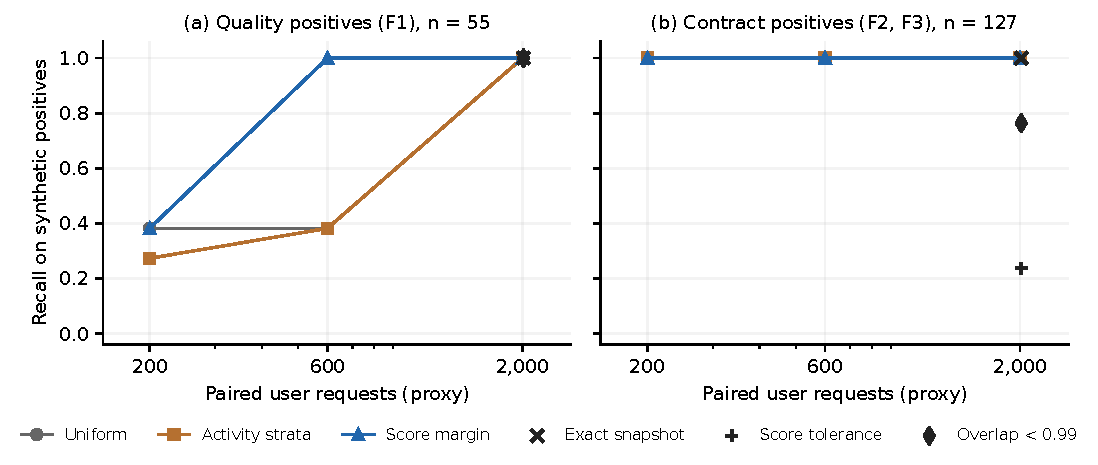
\includegraphics[width=\textwidth]{figures/detection_cost.pdf}
  \caption{Recall against the request proxy at $\delta=0.005$, for quality
    positives (a, all F1) and contract positives (b, F2 and F3). Lines are probe panels by
    selection rule; single markers are full-output change detectors.}
  \label{fig:detection}
\end{figure}

\begin{figure}[htbp]
  \centering
  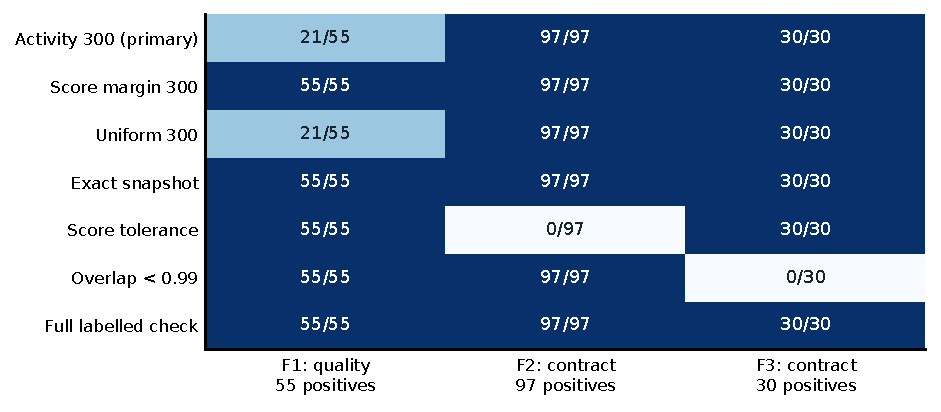
\includegraphics[width=.8\textwidth]{figures/synthetic_recall_v2.pdf}
  \caption{Detected and total positives by fault class at $\delta=0.005$.
    Separating quality positives (F1) from contract positives (F2, F3) shows
    what the aggregate recall conceals.}
  \label{fig:synthetic}
\end{figure}

\paragraph{Tolerance and pipeline.} Table~\ref{tab:syn-deltas} repeats the main
detectors at the three tolerances. The set of positives changes with the
tolerance (\synPositivesLow{} at 0.002, \synPositivesHigh{} at 0.010) because
fewer F1 outputs are harmful at a larger tolerance. At $\delta=0.010$ every
300-user panel labels all 15 remaining F1 positives inconclusive.
Positives from the same pipeline
are not independent, so Table~\ref{tab:syn-pipeline} splits recall by
pipeline. The primary panel's misses are all item-ID swaps in the reference
item-kNN.

\begin{table}[htbp]
  \centering\small
  \caption{Detected and total synthetic positives (recall) at the three
    tolerances.}
  \label{tab:syn-deltas}
  \begin{tabular}{@{}lccc@{}}
    \toprule
    Detector & $\delta=0.002$ & $\delta=0.005$ & $\delta=0.010$ \\
    \midrule
    \tablebody{tab_x_syn_deltas}
    \bottomrule
  \end{tabular}
\end{table}

\begin{table}[htbp]
  \centering
  \caption{Detected and total synthetic positives by pipeline at
    $\delta=0.005$.}
  \label{tab:syn-pipeline}
  \footnotesize\setlength{\tabcolsep}{4pt}
  \begin{tabular}{@{}llccccc@{}}
    \toprule
    ID & Pipeline & Activity 300 & Margin 300 & Uniform 300 & Overlap, lenient & Score tol. \\
    \midrule
    \tablebody{tab_x_syn_pipeline}
    \bottomrule
  \end{tabular}
\end{table}

\paragraph{Answer to RQ3.} At the primary margin, the 300-user activity panel
detected \synPrimaryFOne{} of \synFOne{} quality faults and all
\synContractPositives{} contract faults. The secondary margin panel detected
all positives at the same paired-user count, with the three no-fault alarms
described above. Output-change
detectors cannot separate churn from harm: the strict ones alarm on benign
upgrades, and the tolerant ones miss a fault class. These results describe
constructed faults on real outputs, not the detection of real harmful
upgrades, of which the study observed none.

\FloatBarrier

% ---------------------------------------------------------------------------
\section{Mechanisms and Case Studies}
\label{sec:mechanisms}

\subsection{M1: Exact ties in selection and neighbour pruning}
\label{sec:m1}

The development transition N1 changes NumPy from 1.26.4 to 2.0.2. In
float32 reference item-kNN inference, 3 of 1{,}007 users received a
different native top-10 list despite identical scores, seen masks and
canonical rankings. Replays of native selection on the same frozen score,
mask and item-ID arrays matched the original lists on both versions.
Rollback recovered the baseline lists and reapplication recovered the
upgraded lists. The lock diff isolates NumPy, whose release notes describe
changed outcomes for unstable sort and partition operations
\citep{numpy2releasenotes}.

Table~\ref{tab:ties} connects this to Section~\ref{sec:ties}. In each affected
primary inference comparison, three users have a tie that crosses the cutoff, and
exactly those three users change. Their tie blocks hold between 3{,}578 and
3{,}650 of the 3{,}655 catalogue items: these are users for whom almost every
eligible item has the same score. The two deterministic routines select
different subsets from these blocks, and the measured loss is $0$ with
interval $[0,0]$ on the primary split.

\begin{table}[htbp]
  \centering\small
  \caption{Cutoff ties in the inference comparisons affected by M1. Crossing:
    users whose tie block crosses the top-10 cutoff (Equation~\ref{eq:tieblock}).
    Block: range of $|T_u|$ for those users. Changed: users whose native
    top-10 list differs between sides.}
  \label{tab:ties}
  \begin{tabular}{@{}lrrrrc@{}}
    \toprule
    Case & Users & Crossing & Block size & Changed & Canonical equal \\
    \midrule
    \tablebody{tab_x_ties}
    \bottomrule
  \end{tabular}
\end{table}

The same selection mechanism acts upstream during retraining, in the
neighbour pruning of Equation~\eqref{eq:knn}. For N1 float32, both
environments reconstructed identical pre-pruning cosine weights in the same
encounter order. Replaying pruning recovered the original model hashes. Each
of the 734 changed target neighbourhoods exchanged neighbours at an exact
pruning-boundary tie. A different neighbour set changes some scores
substantially (Table~\ref{tab:numeric}), yet lists changed for 0.3\% to 0.4\%
of users and quality not at all. The held-out Q2 bundle includes NumPy 1.26.4
to 2.0.0 and reproduces the selection and fitted-neighbourhood signatures.
The selection effect appears on all three tested CPUs. On MovieLens~20M, with
12{,}388 training items, it produced a positive point loss of
\lossMOneMLtwenty{}, below the smallest declared tolerance.

\subsection{M2: BLAS kernel dispatch during ALS fitting}

In development transition N2, NumPy 2.0.2 and 2.1.3 both bundled OpenBLAS
0.3.27. On host A the older build selected Cooperlake kernels and the
newer build selected SkylakeX (Table~\ref{tab:blas}). Restoring the frozen
factors for inference gave identical results. With fresh training from paired
initial factors, the fitted model was the first changed checkpoint. For
seed~17, forcing \texttt{OPENBLAS\_CORETYPE=SkylakeX} in the older environment
reproduced the newer fitted factors and rankings bit for bit. The held-out Q3
bundle, which includes the NumPy 2.0.0 to 2.1.1 transition, reproduced the N2
fitted model exactly. The core setting is process-wide and may affect
multiple OpenBLAS copies. The replay demonstrates the effect of the forced
core setting in this environment. The available trace does not isolate the
ALS call-site provider or identify the source of the default dispatch
difference between the two same-version bundles.

The observations are consistent with ordinary floating-point
non-associativity \citep{higham2002accuracy}: different kernels may accumulate
the same products in a different order, so intermediate results can differ in
their last bits. ALS feeds each sweep's factors into the next
(Equation~\ref{eq:als}), and after 15 alternating sweeps the two sides differ
by a relative score difference of $1.7\times10^{-3}$, enough to reorder close
scores for 8.48\% of users. The reordering shows no preferred direction: the
loss intervals of all three metrics contain zero
(Table~\ref{tab:secondary}).

\begin{table}[htbp]
  \centering
  \caption{ALS retraining on MovieLens~1M (N2-P2-als): loss, baseline minus
    upgraded, with the primary 95\% paired-seed interval and the sensitivity
    interval that resamples seeds and users. Q3-P2-als and B1-P2-als contain
    the same NumPy 2.0 to 2.1 change and reproduce exactly the same values.}
  \label{tab:secondary}
  \small
  \begin{tabular}{@{}llll@{}}
    \toprule
    Metric & Loss & Paired-seed interval & Seed-and-user bootstrap \\
    \midrule
    \tablebody{tab_x_secondary}
    \bottomrule
  \end{tabular}
\end{table}

\subsection{M3: Bundled BLAS binary and EASE coefficients}

Cornac EASE inverts the regularised Gram matrix of Equation~\eqref{eq:ease}
with \texttt{numpy.linalg.inv}. The N5 and N6 contrasts share the NumPy~2.4.6
environment, which bundles OpenBLAS~0.3.31; the fitted model was bit-identical
across the other tested NumPy builds (OpenBLAS 0.3.29, 0.3.30 and 0.3.34).
% Coefficients recomputed from the saved models (seed 17): max abs 1.30e-15,
% relative L2 3.16e-15. Score diagnostics: 9.9e-14 and 5.1e-16.
The fitted coefficient matrices differ by at most $1.3\times10^{-15}$
(relative $L_2$ difference $3.2\times10^{-15}$), and the downstream scores by
at most $9.9\times10^{-14}$. Top-10 lists were identical.

% results/diagnosis/N5-P6-ease/summary.json, independently audited.
A reciprocal intervention held each NumPy environment fixed and preloaded the
other environment's bundled OpenBLAS binary (Table~\ref{tab:ease}). The fitted
model hash followed the donor binary in both directions, and removing the
preload restored each native hash. Loader traces verified that NumPy's
linear-algebra calls bound to the intended binary. Both libraries reported
the SkylakeX dispatch class; this does not establish identical kernel code
across builds. The experiment attributes the change to the bundled binary,
including its build configuration, for the replayed seed and host. It does not
separate an upstream source change from build options.

\begin{table}[htbp]
  \centering\small
  \caption{Reciprocal OpenBLAS intervention for EASE (seed 17, primary host,
    one thread). Donor identifies the NumPy wheel supplying the BLAS binary;
    S3 shows the first 16 hexadecimal digits of the model checkpoint digest.
    The model follows the donor in both directions and returns on rollback.
    Native top-10 and top-20 lists are identical in all six runs.}
  \label{tab:ease}
  \begin{tabular}{@{}llll@{}}
    \toprule
    NumPy environment & Condition & BLAS donor wheel & S3 digest prefix \\
    \midrule
    \tablebody{tab_ease_intervention}
    \bottomrule
  \end{tabular}
\end{table}

\subsection{M4: A last-bit change in \texttt{log1p}}

The \texttt{implicit} BM25 weighting of Equation~\eqref{eq:bm25} calls
\texttt{log1p}. % protocol/reproducers/README.md.
Hashing each intermediate step of the weighting showed that only the
\texttt{log1p} output, and what follows from it, differs between NumPy 1.26.4
and 2.0.2 on host A: 1{,}073 of the 5{,}186 values (one per training user), by
at most $8.9\times10^{-16}$. This changes the fitted BM25 weights (S3) and the
scores (maximum difference $2.9\times10^{-11}$) but no top-10 list. Running
NumPy~2.0.2 with the 1.26.4 \texttt{log1p} values substituted reproduced the
1.26.4 weights exactly. Switching to legacy type promotion left the result
unchanged. The reproducer and reported hash are retained. The original
intermediate arrays and full replay logs are unavailable in the artifact.
The change is present on both AVX-512 hosts and absent on the AVX2 host.

\subsection{M5: PyTorch on a GPU}

On the T4 GPU, PyTorch~2.10.0 trained a slightly different BPR model than
2.9.1 in five of five seeds, under deterministic settings and frozen inputs
(Table~\ref{tab:gpu}). The change reached the top-20 lists for two seeds and
never the top-10. cuBLAS, cuDNN and the CUDA runtime were unchanged between
the locked environments, while PyTorch, Triton and NVSHMEM versions changed.
Without an operator-level intervention, the evidence supports attribution to
the changed environment bundle, not to a specific PyTorch source change. We
report it as unresolved. The effect is not run-to-run noise: a second Job
reproduced every model digest of the first, and each of its
\rerunGpuDeviceRuns{} runs recorded the device (Tesla~T4, CUDA).

\begin{table}[htbp]
  \centering\small
  \caption{Unresolved GPU extension, separate from the attributed CPU
    mechanisms. The other five declared GPU transitions have identical
    checkpoints. All six completed with equivalent NDCG@10 verdicts.}
  \label{tab:gpu}
  \begin{tabularx}{\textwidth}{@{}lX@{}}
    \toprule
    Field & Recorded observation \\
    \midrule
    Case / device & T1-P7-gpu / NVIDIA Tesla T4 \\
    Treatment & PyTorch 2.9.1 to 2.10.0, with its resolved environment changes \\
    Frozen-model inference & Identical checkpoints \\
    Retraining & Fitted model differs in five paired seeds \\
    Score difference & Maximum absolute difference $4.8\times10^{-6}$ \\
    Ranked output & Top-20 differs in two seeds; top-10 unchanged \\
    Attribution & Unresolved at the environment-bundle level \\
    \bottomrule
  \end{tabularx}
\end{table}

\subsection{Issue-guided leads}

% protocol/cases/issue_guided.yaml.
Table~\ref{tab:leads} summarises the 29 issue-guided leads. Fourteen describe
visible failures and three were reproduced; four could not be reproduced and
eight were not tested, each with a recorded reason. Some labels reflect source
triage or checks on newer releases rather than a local reproduction of the
historical environment, so these are not 29 executed cases. One reproduced
lead is M1. The other two are component effects that did not reach a ranking
in this study. In a frozen synthetic TF-IDF fixture, the released Recommenders
ranking method returned the same self-recommendation under both NumPy
versions. A synthetic sparse fixture with duplicate entries changed the
released \texttt{implicit} normaliser's output under SciPy~1.13.0; SciPy~1.13.1
and rollback to 1.12.0 restored the baseline. The effect cannot reach our
rankings, because MovieLens~1M contains no duplicate user--item pairs, and
SciPy~1.13.0 is not in the systematic selection, which takes the latest patch
of each minor release.

\begin{table}[htbp]
  \centering\small
  \caption{Issue-guided leads by upstream project and closing status. These
    leads informed mechanism hypotheses and are never pooled with the
    systematic collections.}
  \label{tab:leads}
  \begin{tabular}{@{}lrrrrr@{}}
    \toprule
    Project & Reproduced & Visible failure & Not reproducible & Not tested & Total \\
    \midrule
    \tablebody{tab_x_leads}
    \bottomrule
  \end{tabular}
\end{table}

% ---------------------------------------------------------------------------
\section{Practical Guidance}
\label{sec:guidance}

The results support five recommendations. They come from shallow models on
MovieLens data, run on one thread, and should be read with that scope.
\begin{enumerate}
  \item \textbf{Do not judge an upgrade by list churn alone.} A changed top-10
    list after an upgrade was equivalent at the declared tolerances in every
    completed real comparison. Exact-output comparisons and strict overlap
    thresholds alarm on such churn, and even on a tie-order rebuild with no
    fault at all. Churn is not always harmless either: in the Surprise SVD
    no-fault control, a different valid tie order alone moved NDCG@10 by
    0.0033, more than the smallest margin. Judge an upgrade by relevance-based
    quality with an interval and a declared tolerance.
  \item \textbf{Break ties explicitly.} The only mechanism that appeared on
    every tested CPU was tie reordering in unstable selection. Use a
    deterministic secondary key over the full eligible tie block at the
    selection boundary (Equation~\ref{eq:tieblock}), or a full lexicographic
    ranking. Stably sorting only an already selected subset cannot recover
    tied items excluded earlier. We did not benchmark the cost of this repair.
  \item \textbf{Test on the hardware you deploy.} M2--M5 varied with the
    tested host or device. An upgrade that leaves results unchanged on a
    developer's laptop can change them on a server, and the reverse. Record
    the CPU and the BLAS kernel with every result, and repeat upgrade checks
    on the production instruction set. We tested one thread only. With
    multi-threaded BLAS, first check that two runs of the same environment
    still agree, because the comparison depends on that control.
  \item \textbf{Record native libraries and core selection.} EASE changed
    with the bundled OpenBLAS binary. ALS changed under a process-wide core
    override on the primary host. Record native binary identities and
    selected cores alongside the Python package lock (Table~\ref{tab:blas}).
  \item \textbf{Check contracts always, and quality with labels.} Contract
    checks on seen items and finite scores caught every contract fault with as
    few as 100 users. For quality, a score-difference threshold is not a
    substitute for labels (Figure~\ref{fig:perturbation}). On the synthetic
    faults, which we chose ourselves, a 300-user panel selected at the ranking
    boundary detected more quality faults than a uniform or activity panel of
    the same size. It also raised alarms on three no-fault controls, so treat
    its alarms as a reason to run a full evaluation. Measure selection,
    scoring and confirmation time before claiming savings; we did not.
\end{enumerate}
In this study the upgrades that broke a pipeline did so visibly: pin upper
bounds where a dependency has removed aliases, and run the pipeline, not only
the import, after an upgrade. Projects with unpinned requirements meet all of
these changes whenever they install (Figure~\ref{fig:timeline}); projects with
lockfiles meet them when they choose to upgrade.

% ---------------------------------------------------------------------------
\section{Threats to Validity}
\label{sec:threats}

\paragraph{Construct validity.} Offline NDCG@10 on held-out relevance is a
proxy for user-facing quality; an equivalent verdict does not exclude effects
on online behaviour, diversity or fairness. A changed list can matter to a
product even without a quality loss, which is why we report behavioural change
separately. The tolerances are absolute NDCG differences declared before the
held-out runs; equivalence at the tested tolerances does not establish
equivalence at a smaller one. The failure signals configured here were the
process exit status, exceptions and the output contracts. Most upstream test
suites could not run in our harness (Table~\ref{tab:suites}), so
\emph{silent} means in practice that the run completed and its output passed
the contracts. Synthetic faults are constructed outputs rather
than observed upgrade defects. For users a fault touches, the faulted list
comes from a reference ranker and not from the pipeline's own ranker, which
cannot be rerun on faulted scores. The request count is a proxy for cost.

\paragraph{Internal validity.} All completed ranking cases passed a
bit-identical same-environment inference control. Comparisons used frozen,
checksummed inputs. The hyperparameter is selected once, in the baseline
environment, and used on both sides. We did not tune again in the upgraded
environment, so a change in which setting would be selected after an upgrade
is outside what the study observes. The protocol tag records the order of
events in the project repository; it is not a public registration or a
third-party timestamp. A snapshot
transition can change several packages at once; we attribute snapshot effects
through the single-dependency cases they contain. The hosts differ in more
than the processor: the primary host is a laptop running the container under
WSL2, and the others are rented cloud hosts with a different Linux kernel.
The BLAS interventions
establish attribution for the replayed seed and host, not for every seed.
M5 is unresolved. M3 and M4 co-occur with AVX-512 on the tested hosts, but no
instruction-disable intervention isolates that feature. For the EASE replay,
saved digests and loader traces support the donor-binary result, while the
launch-time source and mount record was not archived. The synthetic analysis
was corrected after an audit of its first version: the fault-isolation rule of
Equation~\eqref{eq:isolation} was written after the first results were known,
and its tie-faithful ranker was added after one trial case. The cohort, the
faults, the detectors and the primary configuration were not changed, and the
detection counts of the two versions agree at $\delta=0.005$. Each reported
mechanism rests on a replay whose inputs and output digests are saved, so the
replays can be repeated. How we interpret them has not been reviewed by a
second person.

\paragraph{External validity.} The study covers two MovieLens datasets, eleven
pipeline configurations from five libraries plus two reference
implementations, three CPU types and one GPU type. Systematic release
selection covers January 2024 through October 2026, with a separate
1~November 2026 resolution cutoff for development bundle B1. The reference implementations are small but contain the
idioms through which the mechanisms act. Larger neural recommenders, other
domains (for example e-commerce or news), LensKit, RecBole and other
accelerators were not studied. The study used one thread; multi-threaded BLAS
adds its own nondeterminism. The absence of SciPy, pandas and CPU PyTorch
effects covers only the functions that these eleven configurations call.
Because harm was absent, we cannot estimate how
often harmful silent regressions occur, only that none were supported in the
completed real comparisons. The primary denominator includes failures,
preprocessing and inapplicable configurations, and related transitions share
mechanisms, so a binomial zero-event bound over all \nCases{} cases would be
inappropriate.

\paragraph{Conclusion validity.} The unit of independence is the mechanism,
not the user or the case. Eight mechanisms are too few for prevalence claims
about mechanisms in general, and we make none. Development and held-out cases
are separated; the mechanisms identified in development recurred in the
held-out collection at the versions the diagnosis predicted. Issue-guided
leads were not pooled with the systematic collection. Synthetic positives from
the same base case and pipeline are clustered, which is why recall is also
reported by pipeline.

\paragraph{Artifact and analysis validity.}
The frozen tables report the first rented-host Jobs, which exported reports,
metrics and run metadata but not their arrays. The second Jobs retain the
model, score and ranking arrays of every run (\rerunGigabytes{}~GB,
checksummed) and a device record for each GPU run, and they reproduce the
first Jobs digest for digest (Table~\ref{tab:reruns}), so the rented-host
results can be re-evaluated independently. The interaction-matrix checkpoint
is not archived; it is rebuilt from the frozen data, and its digest is kept.
Hugging Face does not document the processor behind a hardware flavor; the
probe recorded the same CPU models in both rounds. Upstream suites were
screened on the primary host only. The local reporting package contains
the ledger snapshots and inputs used to regenerate the results tables and
figures, with a SHA-256 manifest. The primary estimates, confidence intervals,
and verdicts can be recomputed from the saved per-user metrics. The study
materials await public deposit.

% ---------------------------------------------------------------------------
\section{Conclusion}
\label{sec:conclusion}

Among \nCases{} primary cases, \nChanged{} changed a checkpoint silently and
\nListChanged{} changed a top-10 list. The interventions link these changes
to four mechanisms: unstable tie selection, a BLAS core setting, a bundled
BLAS binary and a last-bit
change in a math function. A GPU extension adds an unresolved training
difference. Every completed real comparison supports offline quality
equivalence at the declared tolerances, on two datasets and four devices,
while the upgrades that broke pipelines crashed or failed to install. The same
NumPy wheel changed results on one processor and left them unchanged on
another, showing that a dependency upgrade can alter native-library behaviour
in a hardware-dependent way. In the synthetic controls, contract checks
detected all contract faults, while the primary labelled panel missed
many quality faults. The maintenance lesson
is to measure numerical differences, ranking differences, contracts and
relevance-based losses separately, and to keep the environment and hardware
evidence needed to explain them. These findings hold for shallow models on
MovieLens data and one thread. Larger neural recommenders, other domains and
multi-threaded execution are the natural next tests: ALS, the one iteratively
trained CPU model that changed, also showed by far the most list churn.

% ---------------------------------------------------------------------------
\section*{Data Availability}
\label{sec:data-availability}

The study materials are retained in the project workspace and have not yet
been deposited in a public archive. They include source code, environment
locks, manifests, frozen protocols, the ledgers of all hosts, comparison
reports, the checksummed array archives of the rented-host reruns, both
versions of the synthetic analysis and diagnostic artifacts.
The paper scripts regenerate the results tables, figures and numerical
macros from saved inputs. The local reproduction package includes checksums
and an inventory of the retained evidence.
Dataset download and preparation scripts verify checksums; the datasets
themselves are not redistributed.

\appendix
\section{Transitions, Snapshots and Run Cost}

\begin{table}[htbp]
  \centering
  \caption{Single-dependency transitions and the outcomes of their primary
    cases. Held fixed: the other pinned numerical dependencies (np: NumPy,
    sp: SciPy, pd: pandas). Chg.: a checkpoint changes.}
  \label{tab:transitions}
  \scriptsize\setlength{\tabcolsep}{3pt}
  \begin{tabular}{@{}llllrrrrrr@{}}
    \toprule
    ID & Package & Old $\rightarrow$ new & Held fixed & Split & Cases & Ident. & Chg. & Fail. & N/A \\
    \midrule
    \tablebody{tab_x_transitions}
    \bottomrule
  \end{tabular}
\end{table}

\begin{table}[htbp]
  \centering
  \caption{Resolved versions of the unpinned requirements at each upload
    cutoff, and the bundle transition that ends at that snapshot (from the
    previous quarterly snapshot; B1 runs from 2024-06-01 to 2026-11-01).}
  \label{tab:snapshots}
  \scriptsize\setlength{\tabcolsep}{4pt}
  \begin{tabular}{@{}lllllrrrr@{}}
    \toprule
    Cutoff & NumPy & SciPy & pandas & implicit & Transition & Cases & Changed & Failed \\
    \midrule
    \tablebody{tab_x_snapshots}
    \bottomrule
  \end{tabular}
\end{table}

\begin{table}[htbp]
  \centering\small
  \caption{Completed runs on the primary host by mode. Wall time includes
    container start. One thread per run.}
  \label{tab:cost}
  \begin{tabular}{@{}lrrrrr@{}}
    \toprule
    Mode & Runs & Median wall (s) & Max wall (s) & Median CPU (s) & Max RSS (MiB) \\
    \midrule
    \tablebody{tab_x_cost}
    \bottomrule
  \end{tabular}
\end{table}

\section{Scale and Split-Sensitivity Results}
\begin{table}[htbp]
  \centering
  \caption{All case--mode comparisons on MovieLens~20M and on the separate
    MovieLens~1M per-user split. Change refers to any checkpoint. Users is
    the mean percentage with changed top-10 lists. Loss is baseline minus
    upgraded NDCG@10 with its primary 95\% interval. Every listed verdict is
    equivalent at all three tolerances; populations are not pooled.}
  \label{tab:extensions}
  \scriptsize\setlength{\tabcolsep}{3pt}
  \begin{tabular}{@{}lllrl@{}}
    \toprule
    Case & Mode & Change & Users\,\% & Loss [95\% interval] \\
    \midrule
    \tablebody{tab_extensions}
    \bottomrule
  \end{tabular}
\end{table}
\clearpage

\bibliographystyle{plainnat}
\bibliography{refs}

\end{document}
